\chapter{Численное моделирование} \label{chapt2}

\section{Теоретическое описание керровских гребенок в микрорезонаторах}

\subsection{Оптическая нелинейность в микрорезонаторах}
Поскольку оптические моды типа шепчущей галереи в резонаторах сочетают малый эффективный объем локализации поля с высокой добротностью, то порог проявления различных нелинейных эффектов оказывается низким \cite{Gorodetsky}. Одним из таких эффектов является нелинейный эффект четырехчастотного взаимодействия, приводящей к формированию оптической гребенки: два фотона переходят в боковые линии (рис. \ref{cascading}). Если накачка достаточно велика, то гребенка формируется благодаря каскадному процессу образования таких боковых линий, как суммы взаимодействий всевозможных 4 фотонов, удовлетворяющим частотным требованиям. Эффект возникает из-за материальной Керровской нелинейности среды.

\begin{figure}
  \centering
%  width=390pt,height=550pt
  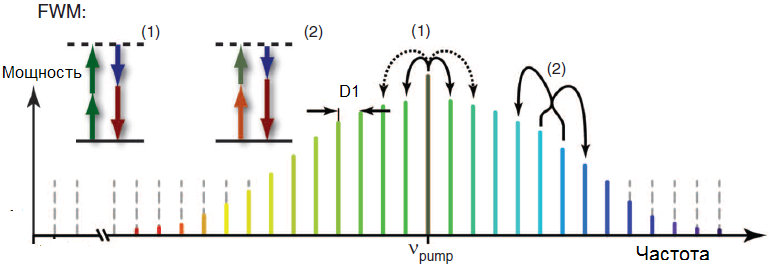
\includegraphics[]{FWM_Science}
  \caption{Эффект четырехчастотного взаимодействия. $(1)$ - вырожденный случай (два фотона одинаковой частоты переходят в фотоны большей и меньшей частоты), $(2)$ - невырожденный случай (все четыре фотона имеют разные частоты)} \label{cascading}
\end{figure}


Описание нелинейных оптических явлений можно проводить разложением вектора поляризации в ряд:
%
\begin{equation}
P(t)=\epsilon_0[\chi^{(1)}E(t)+\chi^{(2)}E^2(t)+\chi^{(3)}E^3(t)+\dots] =P^{(1)}(t)+P^{(2)}(t)+P^{(3)}(t)+\dots,
\end{equation}
%
где $\chi^{(1)}$ -- линейная восприимчивость, $\chi^{(2)},\chi^{(3)},\dots$ -- нелинейные восприимчивости второго, третьего порядков. $P^{(1)}(t),P^{(2)}(t),P^{(3)}(t)$ -- линейная и нелинейные поляризации второго и третьего порядков. Электрическая индукция в среде
%
\begin{equation}
D(t)=\epsilon E(t)=\epsilon_0E(t)+P,
\end{equation}
%
диэлектрическая проницаемость и показатель преломления $n=\sqrt{\epsilon}$ оказываются зависимыми от напряженности поля:
%
\begin{equation}
\epsilon=1+\chi^{(1)}+\chi^{(2)}E(t)+\chi^{(3)}E^2(t)+\dots,
\end{equation}
\begin{equation}
n=n_0+\frac{1}{2n_0}\chi^{(2)}E(t)+\frac{1}{2n_0}\chi^{(3)}E^2(t)+\dots
\end{equation}
%
В общем случае все коэффициенты являются тензорами, связывающими компоненты вектора поляризации со всеми возможными произведениями компонентов вектора \textbf{E}. В кристаллах, обладающих центром симметрии, а также в изотропных веществах из соображений симметрии $\chi^{(2)}=0$ и основной вклад вносит кубическая нелинейность, при которой изменение показателя преломления вещества пропорционально квадрату напряженности электрического поля. Она может быть обусловлена различными механизмами: ориентационным, электронным, стрикционным -- вместе они называются Керровской нелинейностью. Эффект четырехволнового взаимодействия относится к типу эффектов, в которых наведенная поляризация не колеблется с частотой падающего поля \cite{Gorodetsky}.

\subsection{Отдельная мода}
Рассмотрим действие оптической кубической нелинейности на отдельную высокодобротную моду микрорезонатора. Динамические уравнения для амплитуды поля моды можно получить исходя из уравнений электродинамики:
\begin{equation}\label{initial_electrod}
\nabla\times\nabla\times\textbf{E}+\mu_0\frac{\partial^2\textbf{D}}{\partial t^2}=0,
\end{equation}
\begin{equation}\label{D_induction}
\textbf{D}=\epsilon_0\textbf{E}+\textbf{P}.
\end{equation}
Подставим \eqref{D_induction} в \eqref{initial_electrod} получим волновое уравнение в среде в общей форме:
\begin{equation}
\nabla\times\nabla\times\textbf{E}+\frac{1}{c^2}\frac{\partial^2\textbf{E}}{\partial t^2}=-\frac{1}{\epsilon_0c^2}\frac{\partial^2\textbf{P}}{\partial t^2},
\end{equation}
где член в правой части, играющий роль возбуждающей силы позволяет учесть накачку, нелинейность и дисперсию в среде.
Слагаемое
\begin{equation}
\nabla\times\nabla\times\textbf{E}=\nabla(\nabla\cdot \textbf{E})-\nabla^2E,
\end{equation}
в нелинейном случае нельзя свести к одному векторному оператору Лапласа, т.к. $\nabla\cdot\textbf{E}\neq0$ из-за нелинейной связи векторов $\textbf{D}$ и $\textbf{E}$. Но мы все же пренебрегаем этим членом ввиду его малости. Выделим из поляризации линейную часть, тогда волновое уравнение можно записать в виде:
\begin{equation}\label{wave_eq_polarization}
\nabla\times\nabla\times\textbf{E}+\frac{n^2(\omega)}{c^2}\frac{\partial^2\textbf{E}}{\partial t^2} =-\frac{1}{\epsilon_0c^2}\frac{\partial^2\textbf{P}_{NL}}{\partial t^2}-\frac{1}{\epsilon_0c^2}\frac{\partial^2\textbf{P}_{p}}{\partial t^2},
\end{equation}
где $\textbf{P}_{NL}=\epsilon_0\chi^3(\omega=\omega+\omega-\omega)|\textbf{E}|^2\textbf{E}$, а $\textbf{P}_p$ описывает поляризацию, вызванную полем накачки.
Пусть невозбужденное поле некоторой моды (с номером $\mu$) в линейном случае описывается уравнением
\begin{equation}\label{Helmholz}
\nabla\times\nabla\times\textbf{$e_\mu$}-\frac{n^2(\omega)\omega^2}{c^2}\textbf{$e_\mu$}=0,
\end{equation}
и $e_\mu$ нормировано на максимум так, что $max(e_\mu)=1$, $\int|e_\mu|^2dV=V_{eff}$. Представим поле моды в виде:
\begin{equation}
\textbf{E}=\frac{1}{2}[a(t)\textbf{$e_\mu$}(\textbf{r})e^{-i\omega_pt}+\text{к.с.}],
\end{equation}
где $\omega_p$ -- частота гармонической накачки, близкая к собственной частоте $\omega_\mu$.

Подставляя в \eqref{wave_eq_polarization}, домножая его на $e_\mu^*$ и интегрируя по всему объему, получаем, отбрасывая члены второго порядка малости \cite{Gorodetsky}:
\begin{equation}
\frac{\partial a}{\partial t}+[-i\Delta\omega-i\eta|a|^2+\frac{\kappa_0}{2}+\frac{\kappa_c}{2}]a=iF,
\end{equation}
\begin{equation}
\eta=\frac{3\omega_\mu\chi^{(3)}}{8n^2}\frac{V_{eff}}{V_{jj}},
\end{equation}
\begin{equation}
V_{jj}=\frac{(\int_V|e_\mu|^2dV)^2}{\int_V|e_\mu|^4dV}.
\end{equation}
Здесь $\Delta\omega=\omega_p-\omega_\mu$ и формально добавлены собственные потери $\kappa_o=\kappa_a+\kappa_s=\frac{\omega_0}{\frac{1}{Q_0}+\frac{1}{Q_c}}$, включающие потери поглощения $\kappa_a$ и рассеяния $\kappa_s$, которые можно получить, вводя мнимую часть диэлектрической проницаемости, и потери в элемент связи $\kappa_c$ ($Q_0$ - собственная, $Q_c$ - нагруженная добротности резонатора), а $F$ -- обобщенная сила, учитывающая эффективность связи и мощность, попадающую через элемент связи $P_{in}$
\begin{equation}
F=\sqrt{\frac{2P_{\text{in}}\kappa_c}{\epsilon_0\epsilon V_{\text{eff}}}}
\end{equation}
Для мод шепчущей галереи \cite{Gorodetsky} $V_{jj}\simeq 2V_{eff}$.

\subsection{Несколько мод. Система связанных уравнений}
Рассмотрим процесс генерации гребенки, когда лазер накачки с постоянной мощностью изначально отстроен в область более высоких частот от резонансной частоты. Далее отстройка постепенно уменьшается, в некоторый момент достигается граница параметрической генерации и образуется первая пара боковых мод гребенки.

Пусть $\omega_p$ -- частота накачки лазером, $A_\mu$ амплитуды мод, нормированные, т.ч. $|A_\mu|^2$ число квантов в моде $\mu$. Все номера мод определены относительно моды накачки $\mu=0$. Выражение для собственных мод резонатора с частотами с точностью до кубического члена дисперсии \cite{Herr2012}:
\begin{equation}\label{dispersion_eq}
\omega_\mu=\omega_0+D_1\mu+\frac{1}{2}D_2\mu^2+\frac{1}{6}D_3\mu^3,
\end{equation}
где $D_1$ - область свободной дисперсии (ОСД) резонатора, $D_2$ - разница между двумя соседними ОСД на центральной частоте $\omega_0$. Представим теперь решение в виде:
\begin{equation}\label{SMA_E}
E(r,t)=\sum_\mu\frac{1}{2}A_\mu(t)e^{i\omega_\mu t}e_\mu(r)+\frac{1}{2}A_{ext}e^{i\omega_pt}e_0+\text{к.с.}
\end{equation}
где $\mu$ -- номер рассматриваемой моды, определенный набором ортонормированных собственных мод $e_\mu$ с частотой $\omega_\mu$ и амплитудой $A_\mu(t)$. Нормировка здесь выбрана так, чтобы $|A_\mu|^2$ соответствовало числу фотонов в моде. Направление накачки $A_{ext}$ определяется единичным вектором $e_0$. Пространственные и временные части поля разделяются, мода имеет одинаковую амплитуду по всему пространству. Амплитуда моды меняется медленно $|\dot{A}_\mu(t)|\ll2\omega_\mu|A_\mu(t)|$. Внешняя накачка $\omega_p$ близка к резонансной частоте системы. Пренебрегаем зависимостью $n_\mu(\omega)$ и другими типами взаимодействий мод, кроме четырехчастотного. Рассмотрим левую часть \eqref{wave_eq_polarization}, учитывая \eqref{Helmholz}:
%
\begin{equation}
\frac{1}{2}\sum_\mu(\nabla^2A_\mu e^{i\omega_\mu t}e_\mu+\text{к.с.})-\frac{1}{2c^2}\sum_\mu(\ddot{A_\mu}e_\mu e^{i\omega_\mu t}+(i\omega_\mu)^2e^{i\omega_\mu t}A_\mu e_\mu+\text{к.с.})=\sum_\mu i\omega_\mu n^2 \dot{A_\mu}e^{i\omega_\mu t}e_\mu+\text{к.с.}
\end{equation}
%
Домножим на $\frac{1}{2}(e_\mu+e_\mu^*)$ и проинтегрируем по всему пространству, учитывая ортогональность мод:

\begin{equation}
\int(\sum_\mu i\omega_\mu n^2 \dot{A_\mu}e^{i\omega_\mu t}e_\mu+\text{к.с.})e_\mu dV=\frac{i\hbar\omega_\mu^2}{2\epsilon_0n^2}\dot{A_\mu}e^{i\omega_\mu t}+\text{к.с.}
\end{equation}

Для правой части \eqref{wave_eq_polarization} после возведения в куб и домножения на $\frac{1}{2}(e_\mu+e_\mu^*)$ оставляем члены вида $e_\alpha e_\beta e_\gamma^* e_\mu^* e^{i(\omega_\alpha+\omega_\beta-\omega_\gamma-\omega_\mu)t}$

Окончательно можно получить выражения, определяющие динамику амплитуд \cite{Herr2012}\cite{Chembo2010pra}.
\begin{equation}\label{set_am}
\frac{\partial A_\mu}{\partial t}=-\frac{k}{2}A_\mu+\delta_{\mu 0}\sqrt{k_{ext}}se^{-i(\omega_p-\omega_0)t}+ig\sum_{\mu^\prime,\mu^{\prime\prime},\mu^{\prime\prime\prime}} \Lambda D A_{\mu^\prime}A_{\mu^{\prime\prime}}A_{\mu^{\prime\prime\prime}}^*e^{-i(\omega_{\mu^\prime}+\omega_{\mu^{\prime\prime}}-\omega_{\mu^{\prime\prime\prime}}-\omega_\mu)t},
\end{equation}
где $\kappa=\kappa_0+\kappa_{ext}$ - формально добавленные потери в резонаторе как сумма внутренних потерь $\kappa_0$ и связи с волокном $\kappa_{ext}$. Начальная фаза накачки $0$, $s=\sqrt{P_{in}/\hbar\omega_0}$ описывает амплитуду накачки $P_{in}$, $\delta_{\mu0}$ -- символ Кронекера. $D=2$ при $\mu^\prime\neq\mu^{\prime\prime}$, в других случаях $D=1$.
\begin{equation}
\Lambda=\frac{\int e_{\mu^\prime}e_{\mu^{\prime\prime}}e_{\mu^{\prime\prime\prime}}^*e_\mu^*dV}{\int|e_\mu|^4dV}
\end{equation}

Коэффициент нелинейной связи:
\begin{equation}
g=\frac{\hbar\omega_0^2cn_2}{n_0^2V_{eff}}
\end{equation}
описывает кубическую нелинейность среды с показателем преломления $n_0$, нелинейной частью показателя преломления $n_2$, эффективным нелинейным объемом резонатора $V_{eff}$. Физически $g$ показывает сдвиг частоты каждого фотона из-за керровской нелинейности среды. Для четырехчастотного взаимодействия $\hbar\omega+\hbar\omega^\prime\rightarrow\hbar\omega^{\prime\prime}+\hbar\omega^{\prime\prime\prime}$. Это условие всегда выполняется для эквидистантных мод, однако для мод шепчущей галереи (МШГ) четырехчастотное взаимодействие возможно при $|\omega+\omega^\prime-\omega^{\prime\prime}-\omega^{\prime\prime\prime}|\ll\Delta\omega\mu$. Поэтому суммирование проводится по всем индексам, удовлетворяющим $\mu=\mu^\prime+\mu^{\prime\prime}-\mu^{\prime\prime\prime}$.

В \cite{Matsko2005} показывается, что уравнение \eqref{set_am} можно получить, решая задачу с нелинейным Гамильтонианом.

Систему \eqref{set_am} можно переписать, убрав явную временную зависимость в правой части, и перенормировать все переменные и коэффициенты в единицах ширины резонансов $\kappa/2$, сделав их безразмерными \cite{Herr2012}. Получим:
\begin{equation}
f=\sqrt{\frac{8\eta g}{\kappa^2s}},
\end{equation}
\begin{equation}
d_2=\frac{D_2}{\kappa},
\end{equation}
\begin{equation}
\zeta_\mu=\frac{2(\omega_\mu-\omega_p-\mu D_1)}{\kappa}=\zeta_0+d_2\mu^2,
\end{equation}
\begin{equation}
\tau=\frac{\kappa t}{2},
\end{equation}
\begin{equation}\label{normirovka}
a_\mu=A_\mu\sqrt{\frac{2g}{k}}e^{-i(\omega_\mu-\omega_p-\mu D_1)t},
\end{equation}
\begin{equation}
\eta=\frac{k_{ext}}{k}=\frac{1}{2}.
\end{equation}
Окончательно получим систему уравнений для численного моделирования:

\fbox{
\begin{minipage}{6in}
\begin{equation}\label{compute_eq}
\frac{\partial a_\mu}{\partial \tau}=-[1+i\zeta_{\mu}]a_\mu+i\sum_{\mu^\prime\le\mu^{\prime\prime}} (2-\delta_{\mu^\prime\mu^{\prime\prime}})a_{\mu^\prime}a_{\mu^{\prime\prime}}a_{\mu^\prime+\mu^{\prime\prime}-\mu}^*+\delta_{0\mu}f.
\end{equation}
\end{minipage}}

\subsection{Уравнение Луджиато-Лефевера}

Задачу можно рассматривать в пространственно-временном представлении. Система в этом виде описывается уравнением Луджиато-Лефевера (LLE) \cite{Lugiato1987}. Это уравнение получается из нелинейного уравнения Шредингера (НУШ) добавлением слагаемых, отвечающих за диссипацию и накачку. Можно сказать, что оно же является частным случаем комплексного уравнения Гинзбурга-Ландау \cite{Akhmediev2005}. НУШ описывает распространение коротких световых импульсов в нелинейной среде с дисперсией \cite{Boyd2008}. НУШ является интегрируемой системой, для поиска решений которой используется метод обратной задачи рассеяния \cite{Akhmediev2003}. Уравнение Луджиато-Лефевера не является интегрируемой системой. Вывод уравнения LLE дан в \cite{Matsko2011},\cite{Chembo2013}.

Рассмотрим медленно меняющуюся амплитуду суммарного поля:
\begin{equation}\label{total_field}
A(\phi,t)=\sum_\mu A_\mu(t)e^{i(\omega_\mu-\omega_0)t-i(\mu-\mu_0)\phi},
\end{equation}
где $\phi=[-\pi,\pi]$ азимутальный угол. Частные производные:

\begin{equation}\label{partial_t}
\frac{\partial A}{\partial t}=\sum_\mu(\dot{A_\mu}+i(\omega_\mu-\omega_0)A_\mu)e^{i(\omega_\mu-\omega_0)t-i(\mu-\mu_0)\phi},
\end{equation}
\begin{equation}\label{partial_phi}
i^n\frac{\partial^n A}{\partial \phi^n}=\sum_\mu(\mu-\mu_0)^n A_\mu e^{i(\omega_\mu-\omega_0)t-i(\mu-\mu_0)\phi}.
\end{equation}

Ограничиваясь вырожденным случаем $D=1$ подставим \eqref{total_field}-\eqref{partial_phi} в \eqref{set_am}. Производя замену $d_2=D_2/\kappa$, $\theta=\phi\sqrt{\frac{1}{2d_2}}$, $\tau=\kappa t/2$, $\psi(\tau,\theta)=\sum a_\mu(\tau)e^{i\mu\theta}$ получим:

\fbox{
\begin{minipage}{6in}
\begin{equation}\label{LLE}
i\frac{\partial \psi}{\partial \tau}+\frac{1}{2}\frac{\partial^2 \psi}{\partial \theta^2}+|\psi|^2\psi=(-i+\zeta_0)\psi+if,
\end{equation}
\end{minipage}}

где $\zeta_0, f$ совпадают с \eqref{compute_eq}. Для уравнения LLE не известны точные аналитические решения. Для численного решения существует несколько способов. Так, для стационарного случая \cite{Akhmediev2005} $\frac{\partial \psi}{\partial \tau}=0$ делается Фурье преобразование, полученная система алгебраических уравнений решается методом Ньютона. Другим используемым методом является Фурье метод расщепления по параметрам (Split Step Fourier Method - SSFM).

\section{Численные методы исследования}

\subsection{Метод Рунге-Кутты}
Уравнения для моделирования \eqref{compute_eq} представляет собой систему обыкновенных дифференциальных уравнений первого порядка. Для численного решения обыкновенных дифференциальных уравнений существуют метод Рунге-Кутты, экстраполяционный метод Ричардсона, метод предиктор-корректор и др \cite{Press2002}.

Метод предиктор-корректор хорошо работает для гладких функций. В нем сохраняются все предыдущие рассчитанные значения функции и используются для оценки значения на следующем шаге. В методе Ричардсона используются экстраполяция рассчитанного значения функции к другому значению, которое получилось бы, если бы шаг сетки был меньше текущего. Эти методы сложнее в реализации и требуют большей вычислительной мощности.

В работе использовался широко известный метод Рунге-Кутты. Рассмотрим систему:
%
\begin{equation}
\frac{dy_i(x)}{dx}=f_i(x,y_1,\dots,y_N),\quad i=1,\dots,N,
\end{equation}
%
где функции $f_i$ известны. Заданы начальные условия $y_i(x_s)$, требуется найти $y_i(x_f)$ в конечной точке или во всех точках сетки.

Наиболее часто используется метод Рунге-Кутты 4 порядка (4ый порядок точности). Используется фиксированный шаг $h$ по $x$. Для проверки точности работы алгоритма можно сравнивать результаты, полученные при величинах шага $h$ и $\frac{h}{2}$. Такое сравнение требует значительного вычислительного времени, поэтому лучше ввести адаптивный контроль за работой алгоритма, изменять размер шага во время счета и следить за полученной ошибкой. Фелберг \cite{Press2002} предложил метод пятого порядка с 6 вычислениями функции, т.ч. другая комбинация этих функций дает метод четвертого порядка точности. Разница между двумя вычисленными $y(x+h)$ используется для оценки ошибки и корректировки шага. Общий вид формул метода Рунге-Кутты пятого порядка:
\begin{equation}
k_1=hf(x_n,y_n),
\end{equation}
\begin{equation}
\begin{split}
k_2=hf(x_n+a_2h,y_n+b_{21}k_1),\\
\dots
\end{split}
\end{equation}
\begin{equation}
k_6=hf(x_n+a_6h,y_n+b_{61}k_1+\dots+b_{65}k_5),
\end{equation}
\begin{equation}
y_{n+1}=y_n+c_1k_1+c_2k_2+c_3k_3+c_4k_4+c_5k_5+c_6k_6+O(h^6).
\end{equation}
Формула для четвертого порядка:
\begin{equation}
y_{n+1}^*=y_n+c_1^*k_1+c_2^*k_2+c_3^*k_3+c_4^*k_4+c_5^*k_5+c_6^*k_6+O(h^5).
\end{equation}
Ошибка выражается как:
\begin{equation}
\Delta\equiv y_{n+1}-y_{n+1}^*=\sum_{i=1}^6(c_i-c_i^*)k_i.
\end{equation}
Значения коэффициентов, полученных Cash-Karp \ref{Cash_Karp}, \cite{Press2002}:

\begin{table} [htbp]% Пример записи таблицы с номером, но без отображаемого наименования
	\centering
	\parbox{15cm}{% чтобы лучше смотрелось, подбирается самостоятельно
        %\captionsetup{format=tablenocaption}% должен стоять до самого caption
        \caption{Cash-Karp коэффициенты}%
        \label{Cash_Karp}%

\begin{tabular}{||c|c|c|c|c|c|c|c|c||}
%\hline
%\multline{Cash-Karp коэффициенты}
\hline
i & $a_i$ & & & $b_{ij}$ & & & $c_i$ & $c_i^*$\\
\hline
$1$ & & & & & & & $\frac{37}{378}$ & $\frac{2825}{27648}$\\
\hline
$2$ & $\frac{1}{5}$ & $\frac{1}{5}$ & & & & & $0$ & $0$\\
\hline
$3$ & $\frac{3}{10}$ & $\frac{3}{40}$ & $\frac{9}{40}$ & & & & $\frac{250}{621}$ & $\frac{18575}{48384}$\\
\hline
$4$ & $\frac{3}{5}$ & $\frac{3}{10}$ & $-\frac{9}{10}$ & $\frac{6}{5}$ & & & $\frac{125}{594}$ & $\frac{13525}{55296}$\\
\hline
$5$ & 1 & $-\frac{11}{54}$ & $\frac{5}{2}$ & $-\frac{70}{27}$ & $\frac{35}{27}$ & & $0$ & $\frac{277}{14336}$\\
\hline
$6$ & $\frac{7}{8}$ & $\frac{1631}{55296}$ & $\frac{175}{512}$ & $\frac{575}{13824}$ & $\frac{44275}{110592}$ & $\frac{253}{4096}$ & $\frac{512}{1771}$ & $\frac{1}{4}$\\
\hline
& $j=$ & 1 & 2 & 3 & 4 & 5 & & \\
\hline
\end{tabular}
}
\end{table}

Введем требуемую точность $\Delta_0$, если при шаге $h_1$ получилась ошибка $\Delta_1$, то  \cite{Press2002}:
\begin{equation}\label{h_steps}
h_o=h_1\left|\frac{\Delta_0}{\Delta_1}\right|^{0.2}.
\end{equation}
Если $\Delta_1 > \Delta_0$, то \eqref{h_steps} показывает насколько нужно уменьшить шаг и повторить расчет текущего шага. Если $\Delta_1 < \Delta_0$, то \eqref{h_steps} показывает насколько можно увеличить шаг для следующего вычисления. Поскольку $\Delta_0$ -- вектор требуемой точности, то сравнение можно проводить по отклонению каждого элемента.

%\begin{wrapfigure}{l}{0.7\linewidth}
%  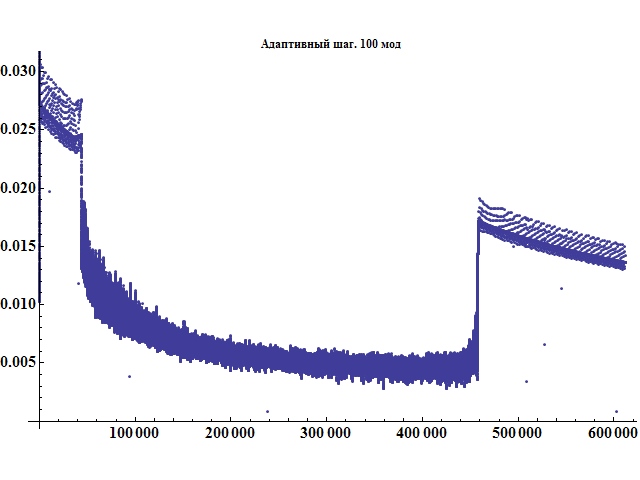
\includegraphics[scale = 0.5]{adaptive_step_100}
%\caption{Зависимость величины адаптивного шага от номера итерации} \label{adaptive}
%\end{wrapfigure}

В программе был добавлен параметр минимальный шаг, ниже которого адаптивное уменьшение запрещено - программа переходит к расчету на следующий узел времени. На практике в большинстве симуляций адаптивность работала на увеличение шага на гладких участках амплитудных кривых, и на уменьшение шага в областях хаотического режима. Количество повторных пересчетов с уменьшенным шагом в среднем составляло около $10\%$ от общего числа шагов по времени.
%Рис. \ref{adaptive} показывает величину шага от его номера.

Адекватность использования метода Рунге-Кутты была проверена хорошим совпадением результатов численного моделирования и эксперимента \cite{Herr2014}. Однако по результатам симуляции видно, что решение чувствительно к малым изменениям параметров. Области генерации могут отличаться даже при новом случайном затравочном шуме в каждой моде.

\subsection{Фурье метод расщепления по параметрам (SSFM)}
Для решения НУШ наиболее быстрым является Фурье метод расщепления по параметрам. Применим его к уравнению Луджиато-Лефевера:
\begin{equation}
i\frac{\partial \psi}{\partial t}+\frac{1}{2}\frac{\partial^2 \psi}{\partial \theta^2}+|\psi|^2\psi=(-i+\zeta_0)\psi+if.
\end{equation}
Выделим линейную $\hat{L}$ и нелинейную $\hat{N}$ части оператора:
\begin{equation}
\hat{N}=i|\psi|^2\psi+f,
\end{equation}
\begin{equation}
\hat{L}=\frac{i}{2}\frac{\partial^2\psi}{\partial \theta^2}-(i\zeta_0+1)\psi.
\end{equation}
Решение на следующем шаге по времени дается выражением:
\begin{equation}
\psi(\theta,t+\tau)\approx\exp (i\tau(\hat{L}+\hat{N}))\psi(\theta,t).
\end{equation}
Это выражение является точным, если $|\psi|^2=const$. Далее происходит разделение по времени:
\begin{equation}
\exp (i\tau(\hat{L}+\hat{N}))\psi(\theta,t)
\approx\exp(i\tau\hat{L})\times\exp(i\tau\hat{N})\psi(\theta,t).
\end{equation}
Это выражение является точным, если $\hat{L}$ и $\hat{N}$ коммутируют. Данную схему можно рассматривать как последовательное решение уравнения для нелинейного оператора \eqref{nonlinear_split_eq}, подстановку полученного значения в \eqref{linear_split_eq} начальным условием. Далее решается уравнение для линейного оператора, решение подставляется начальным условием обратно в \eqref{nonlinear_split_eq}, процедура повторяется.
\begin{equation}\label{nonlinear_split_eq}
\psi_t=\hat{N}\psi,
\end{equation}
\begin{equation}
\tilde{\psi}(\theta,t+\tau)=C\exp(i|\psi|^2\tau)-\frac{f}{i|\psi|^2},
\end{equation}
\begin{equation}\label{linear_split_eq}
\psi_t=\hat{L}\psi,
\end{equation}
\begin{equation}
\psi(\theta,t+\tau)=F.T^{-1}[\exp(-\tau(ik^2+i\zeta_0+1))F.T.[\tilde{\psi}(\theta,t+\tau)]].
\end{equation}

\subsection{Ускорение вычислений для системы связанных уравнений}
Пусть гребенка состоит из $2K+1$ мод, тогда количество нелинейных членов в сумме в \eqref{compute_eq} для всех уравнений равно:
\begin{equation}
\frac{1}{3}(K+1)(8K^2+7+3).
\end{equation}
Время счета для всех мод $T\varpropto K^3+O(K^2)$. Время счета однопоточной программы может быть значительным (больше суток) уже при $K=200$, поэтому возникла необходимость ускорить вычисления путем распараллеливания.

Существуют методы распараллеливания на CPU, использующие POSIX-треды операционной системы с моделью общей памяти (shared-memory). Другой способ - использовать протокол MPI (Message Passing Interface) и модель распределенной памяти (distributed memory). На вычислительном кластере МГУ возможен запуск программ, написанных на языке C или Fortran с использованием MPI библиотек.

Была написана программа на языке C с использованием стандарта MPI, которая реализует метод Рунге-Кутты с адаптивным шагом для уравнения \eqref{compute_eq}. В программе предусмотрена перестройка частоты накачки, рост амплитуды накачки во времени, все входящие в уравнение коэффициенты настраиваются. Результатом работы программы являются зависимости амплитуд мод от отстройки накачки (меняющейся во времени).

Сумма в правой части \eqref{compute_eq} $\sum_{\mu^\prime\le\mu^{\prime\prime}} (2-\delta_{\mu^\prime\mu^{\prime\prime}})a_{\mu^\prime}a_{\mu^{\prime\prime}}a_{\mu^\prime+\mu^{\prime\prime}-\mu}^*$ считается параллельно на нескольких CPU. Каждый из них считает суммы для определенный набора своих мод $\mu$. Корневой процесс (root) рассылает и получает массив амплитуд $a_i$ от других процессов. Далее root рассчитывает значение функции на следующем шаге методом Рунге-Кутта.

Программа была скомпилирована и запущена на ubuntu (реализация OpenMPI-1.6.3), Windows (реализация MPICH2 32bit и 64bit версии) и на суперкомпьютере Ломоносов (OpenMPI-1.5.5). На локальном компьютере быстрее всего работала 64 битная версия под Windows, хотя linux версия запускалась в виртуальной машине. На Ломоносове при равном количестве процессоров программа считает быстрее, чем на ноутбуке. Однако существуют ограничения для пользователя - время счета не более 3 суток, максимальное число процессоров около 100. При таких ограничениях не удалось провести симуляцию для 1000 мод.

На рис. \ref{bechmarking} представлена зависимость времени счета для $200$ мод от количества задействованных процессоров. Заметного улучшения производительности не наблюдается уже при 40 и более процессорах. Это можно объяснить тем, что суммы в нелинейных членах считаются для $200$ мод достаточно быстро, корневой процесс, считающий сам метод Рунге-Кутты, не успевает вычислять и рассылать значения массива мод на новом шаге по времени. Дочерние процессы в это время бездействуют.
%\begin{wrapfigure}{l}{0.7\linewidth}
%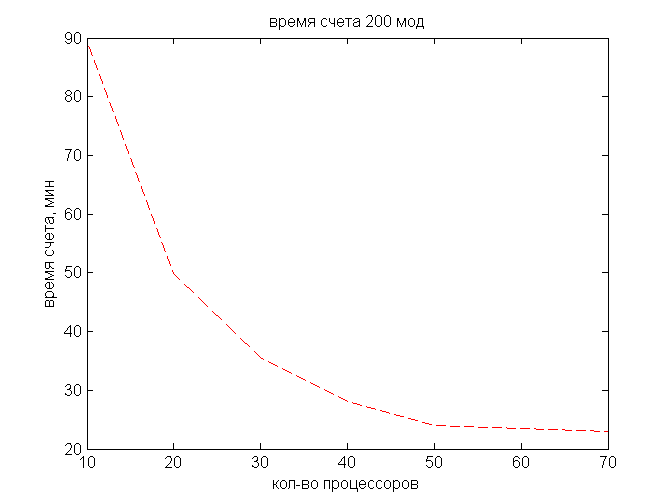
\includegraphics[scale = 0.6]{benchmarking}
%\caption{Ускорение счета} \label{bechmarking}
%\end{wrapfigure}

\begin{figure}
 \centering
 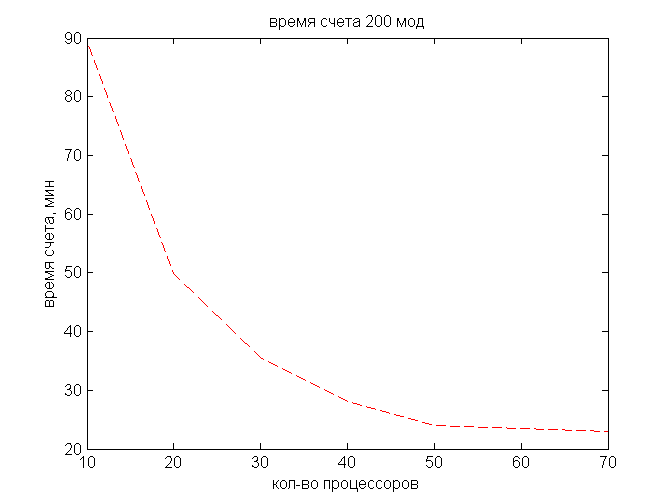
\includegraphics[scale = 0.8]{benchmarking}
 \caption{Ускорение счета} \label{bechmarking}
\end{figure}

В целом время счета нелинейно зависит от диапазона перестройки и сценария симуляции. Заранее оценить его для запуска на кластере проблематично.

Существенное сокращение времени счета было достигнуто методом, предложенным в статье \cite{Hansson2014oc}. Сумма в правой части \eqref{compute_eq} преобразуется с хорошей точностью к виду:
\begin{equation}\label{wabnitz_summation}
\sum_{\mu^\prime\le\mu^{\prime\prime}} (2-\delta_{\mu^\prime\mu^{\prime\prime}})a_{\mu^\prime}a_{\mu^{\prime\prime}}a_{\mu^\prime+\mu^{\prime\prime}-\mu}^*\approx F.T^{-1}[|f_j|^2f_j]
=\frac{1}{N}\sum_{j=0}^{N-1}(|f_j|^2f_j)e^{i2\pi j\mu /N},
\end{equation}
где прямое дискретное преобразование Фурье
\begin{equation}
f_j=F.T[a_\mu]=\sum_{j=0}^{N-1}a_\mu e^{-i2\pi j\mu/n}.
\end{equation}

Было проведено численное сравнение двух методов вычисления правой части. Для гладкого спектра, обращающегося в $0$ на концах, совпадение двух результатов хорошее. Для реального спектра, генерируемого в резонаторе, результат, полученный через Фурье преобразование, всегда больше, чем при прямом вычислении суммы. Для мод, близких к центральной моде накачки, относительная ошибка приблизительно постоянна и составляет до $25\%$. Результаты сравнения даны на рис. \ref{ft_vs_sum}.

\begin{figure}
% \centering
 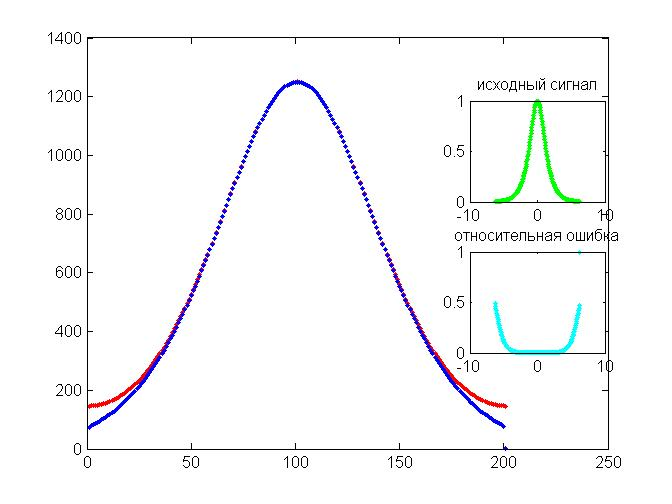
\includegraphics[width = 0.5\textwidth]{ft_vs_sum_sech}
 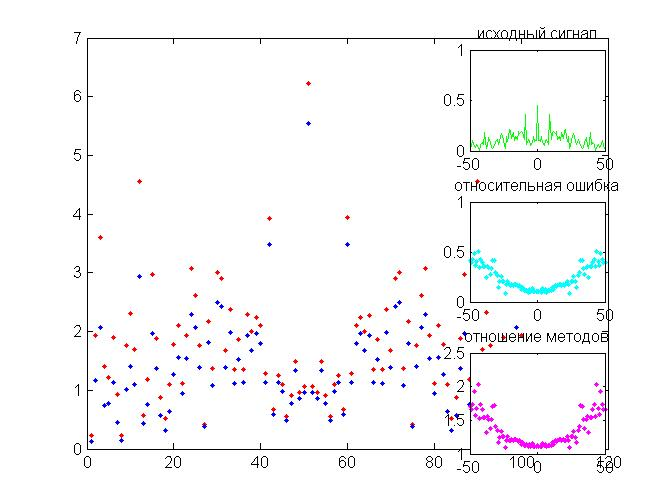
\includegraphics[width = 0.5\textwidth]{ft_vs_sum_comb1}
 \caption{Сравнение методов вычисления суммы. Синим обозначено прямое суммирование. Красным - с использованием \eqref{wabnitz_summation}. Исходный сигнал изображен на верхней вкладке ($sech(x)$ на левом рисунке и спектр реальной гребенки на правом)} \label{ft_vs_sum}
\end{figure}

Несмотря на выявленное отличие, конечные результаты симуляции гребенки двумя методами хорошо совпадают - одинаковы области генераций и наблюдаемые режимы. Тем самым затратное вычисление суммы заменяется на выполнение быстрого прямого и обратного Фурье преобразования. Предыдущая версия программы была переделана под расчет правой части уравнений с использованием стандартных FFT библиотек. Была реализована программа для NVIDIA GPU с использованием библиотеки CuFFT, однако она не дала заметных преимуществ по скорости счета и удобству последующей обработки данных, поэтому основное моделирование проводилось в среде MATLAB.

\section{Результаты моделирования}
\subsection{Используемые программы}
\begin{enumerate}
\item
Многопоточная программа под OpenMPI для симуляции связанных уравнений с суммой в правой части системы \eqref{compute_eq}. Скомпилированная (win32) программа доступна по \href{https://www.dropbox.com/sh/940djjdx3ojcsxy/_1JZsWTqPN/mpi}{ссылке}.
\item
Однопоточная программа для связанных уравнений с Фурье преобразованиями в правой части \eqref{wabnitz_summation}, использующая GPU для быстрого Фурье преобразования. Скомпилированная (win32) программа доступна по \href{https://www.dropbox.com/sh/940djjdx3ojcsxy/n4hBUtto1o/gpu}{ссылке}.
\item
MATLAB программа для связанных уравнений с Фурье преобразованиями в правой части \eqref{wabnitz_summation}.
\item
MATLAB программа для моделирования уравнения LLE \eqref{LLE} методом SSFM.
\item
Пакет Mathematica использовался для решения уравнения LLE \eqref{LLE} методом конечных разностей в функции NDSolve[ ].
\item Графический пользовательский интерфейс, написанный в MATLAB, объединяющий оба метода симуляции и позволяющий задавать параметры системы, сохранять промежуточные результаты на диск для последующей обработки и визуализации. Скриншот интерфейса представлен на рис. \ref{comb_gui}.
\end{enumerate}
\begin{figure}
 \centering
 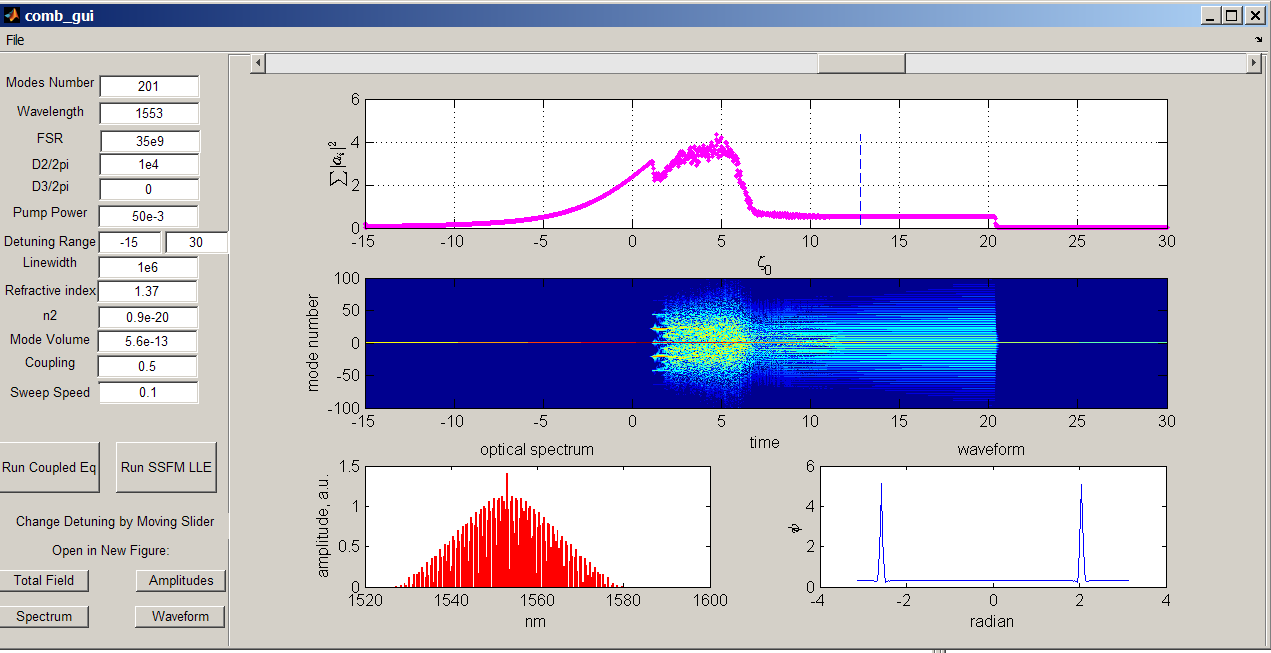
\includegraphics[scale=0.7]{comb_gui}
 \caption{Пользовательский интерфейс программы для численного моделирования CombGUI} \label{comb_gui}
\end{figure}

\subsection{Моделирование по экспериментальным данным}
\label{subsection_experiment}

Рассмотрим дисковый резонатор из $MgF_2$ с параметрами из статьи \cite{Herr2014}. Проверим адекватность теоретической модели путем сравнения результатов моделирования с экспериментальными наблюдениями (экспериментальные данные из \cite{Herr2014}). Начальным условием при решении системы связанных уравнений выступал затравочный шум в каждой моде, имеющий нормальное распределение, - приближение к квантовым нулевым флуктуациям в каждой моде. Используемые параметры:

\begin{equation}
Q_0=Q_c=5\times10^8,
\end{equation}
\begin{equation}
P_0=100\text{ мВт},
\end{equation}
\begin{equation}
\lambda_0=1.553\text{ мкм},
\end{equation}
\begin{equation}
\omega_0=1.213\times10^{15}\text{ Гц},
\end{equation}
\begin{equation}
n_0=1.376,
\end{equation}
\begin{equation}
V_{eff}=V_0=5.6\times10^{-13}\text{ м}^3,
\end{equation}
\begin{equation}
\kappa=\frac{\omega}{Q_0}=1.2\times10^6\text{ Гц},
\end{equation}
\begin{equation}
n_2=0.9\times10^{-20}\frac{\text{м}^2}{\text{Вт}},
\end{equation}
\begin{equation}
g=6.1\times10^{-4},
\end{equation}
\begin{equation}
D_1=2.21\times10^{11}\text{ Гц},
\end{equation}
\begin{equation}
D_2=6.28\times10^4\text{ Гц},
\end{equation}
\begin{equation}
D_3=-800\text{ Гц}.
\end{equation}

Результаты моделирования с помощью многопоточной программы представлены на рис. \ref{100modes},\ref{500modes},\ref{800modes} для $100$, $500$, $800$ мод соответственно.
\begin{figure}
%  \centering
%  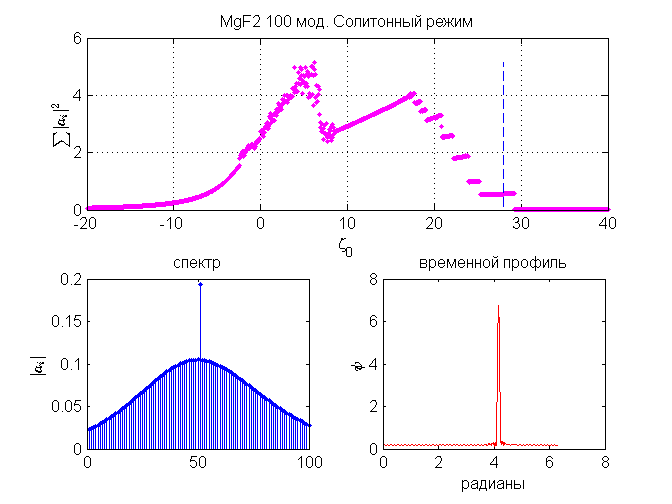
\includegraphics[width = 1\textwidth,height=0.5\textheight]{mgf2_100modes}
 % 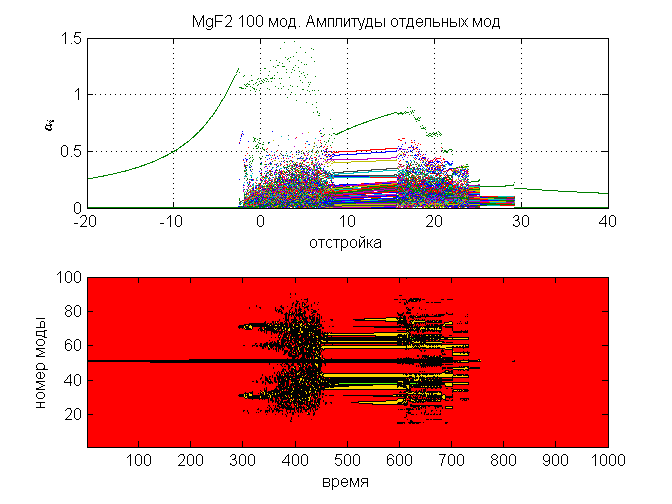
\includegraphics[width = 1\textwidth,height=0.5\textheight]{mgf2_100modes_modal}
  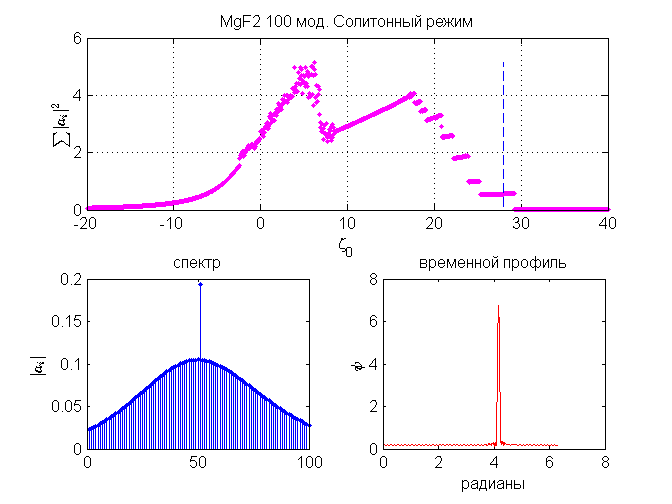
\includegraphics[width = 0.5\textwidth]{mgf2_100modes}
  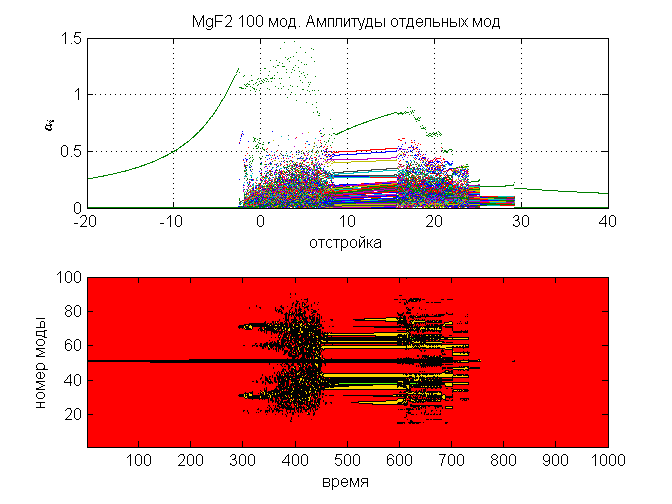
\includegraphics[width = 0.5\textwidth]{mgf2_100modes_modal}
  \caption{Моделирование 100 мод.Резонатор из $MgF_2$. Накачка $100$ мВт} \label{100modes}
\end{figure}

\begin{figure}
%  \centering
%  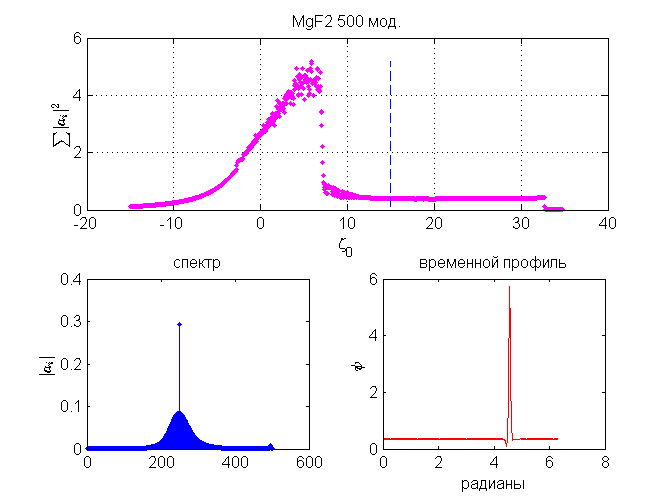
\includegraphics[width = 1\textwidth,height=0.5\textheight]{mgf2_500cluster}
 % 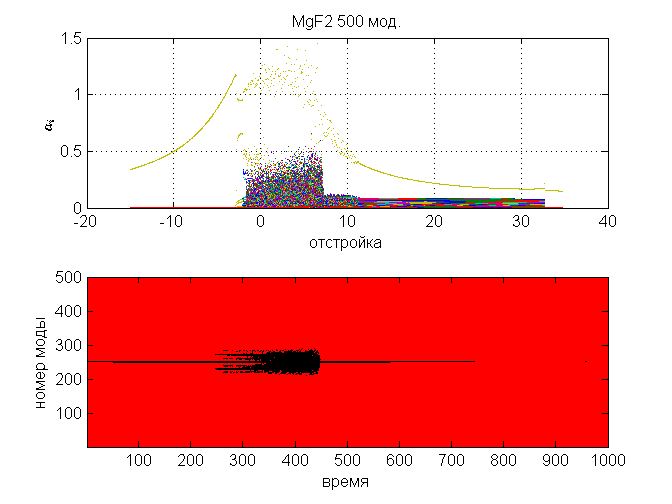
\includegraphics[width = 1\textwidth,height=0.5\textheight]{mgf2_500cluster_modal}
  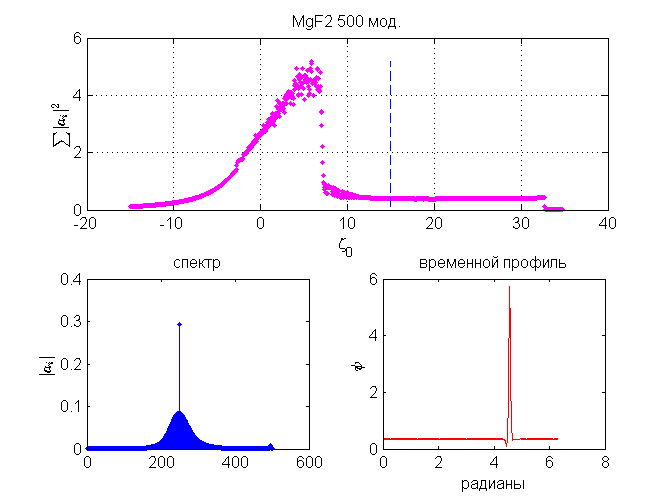
\includegraphics[width = 0.5\textwidth]{mgf2_500cluster}
  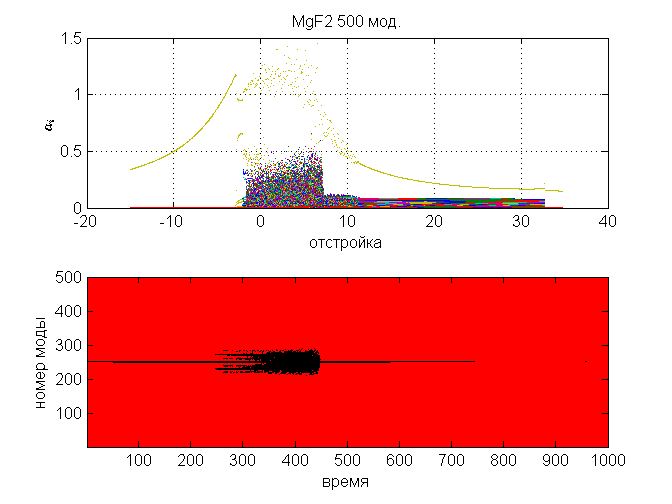
\includegraphics[width = 0.5\textwidth]{mgf2_500cluster_modal}
  \caption{Моделирование 500 мод.Резонатор из $MgF_2$. Накачка $100$ мВт} \label{500modes}
\end{figure}

\begin{figure}
%  \centering
%  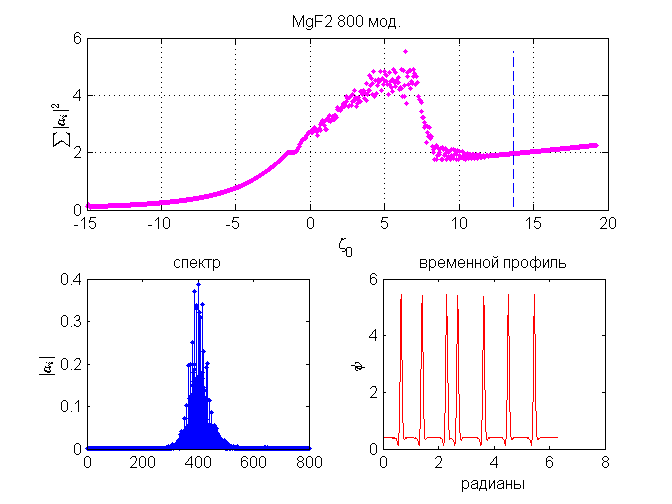
\includegraphics[width = 1\textwidth,height=0.5\textheight]{mgf2_800}
 % 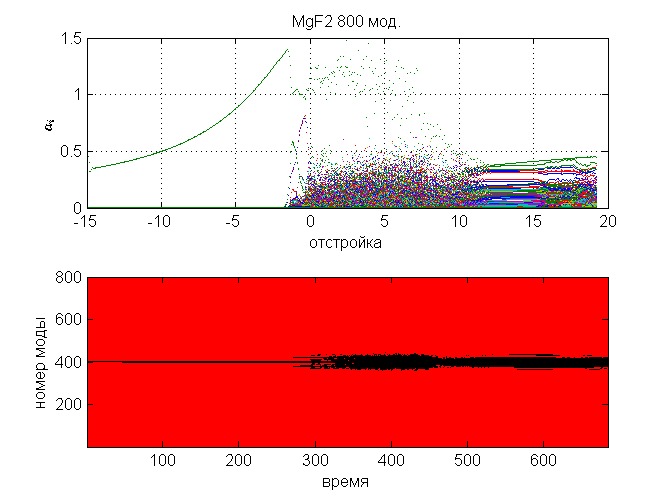
\includegraphics[width = 1\textwidth,height=0.5\textheight]{mgf2_800_modal}
  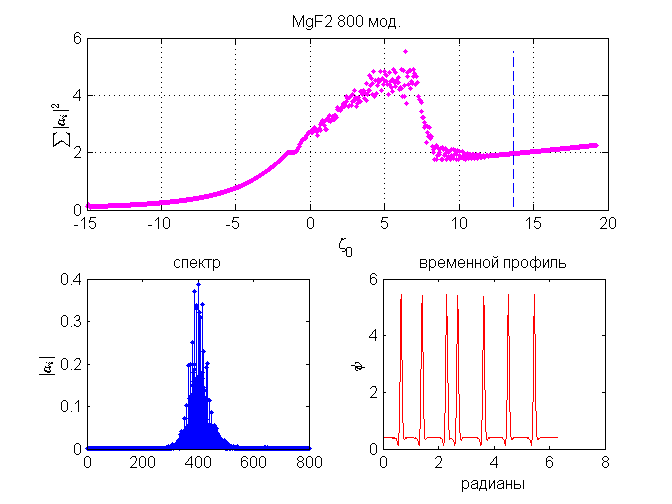
\includegraphics[width = 0.5\textwidth]{mgf2_800}
  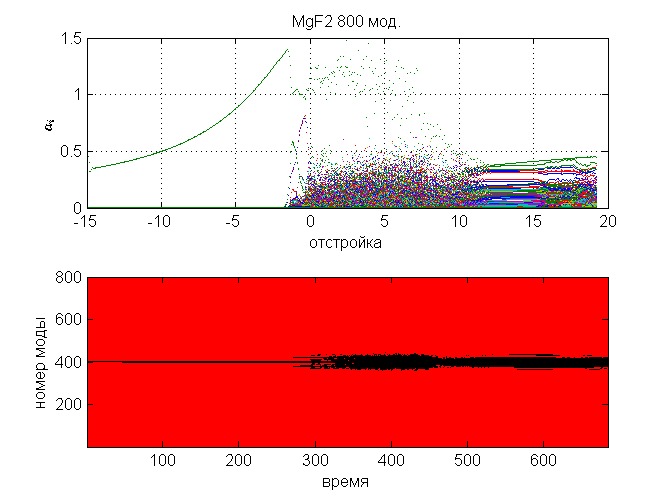
\includegraphics[width = 0.5\textwidth]{mgf2_800_modal}
  \caption{Моделирование 800 мод.Резонатор из $MgF_2$.Накачка $100$ мВт} \label{800modes}
\end{figure}

Число ОСД между соседними модами равно $1$. На левом верхнем графике представлена зависимость суммы квадратов амплитуд всех мод от величины отстройки лазера накачки. Отстройка изменяется линейно от начала до конца диапазона. Ось абсцисс поэтому соответствует временной шкале.  По оси ординат размерность дается нормировкой \eqref{normirovka}, по оси абсцисс отстройка частоты выражена в единицах, т.ч. $1$ соответствует перестройке на $1$ ширину резонансной кривой. Для наглядности приведены аналогичные графики амплитуд отдельных мод, и график, по которому можно понять какие номера мод были возбуждены в данный момент (правый рисунок). Синим цветом дан график спектра - зависимость модуля амплитуды от номера моды при данной отстройке. Текущая отстройка обозначена вертикальным пунктиром на верхнем графике. Красным показан пространственно-временной профиль $\psi(\tau,\Phi)=\sum a_\mu(\tau)e^{i\mu\Phi}$ при той же отстройке.

На всех трех графиках ($100$, $500$, $800$ мод) наблюдается сначала генерация только моды накачки, потом неустойчивая генерация гребенки, носящая хаотический характер. Далее при изменении отстройки возникают чередующиеся области стабильной и нестабильной генерации. В областях стабильной генерации возникают N импульсов (в зависимости от числа рассматриваемых мод), в следующей области N-1 и так далее. Наиболее интересна область генерации одного импульса (солитона), распространяющегося по экватору резонатора. Эта область наблюдалась экспериментально \cite{Herr2014}. Видны отличия между симуляциями $100$, $500$, $800$ мод: из хаотического режима гребенка переходит в устойчивые режимы с разным числом импульсов ($8$, $1$, $7$ соответственно), это связано с различными начальными условиям, затравочными шумаим. Также видно, что моды с номерами, удаленными от центральной моды накачки более, чем на $100$, не возбуждаются (или возбуждаются крайне слабо), что говорит о зависимости ширины гребенки от величины дисперсии второго порядка \cite{Brasch2016}. При большой по модулю аномальной дисперсии генерация широкой гребенки невозможна.

В целом результаты моделирования хорошо соответствуют эксперименту: ступенчатый вид зависимости суммы квадратов амплитуд всех мод от величины отстройки лазера накачки непосредственно наблюдался.

Рис. \ref{caf2} дает результат моделирования эксперимента из статьи \cite{Savchenkov2011}, в котором использовался сфероидальный резонатор из $CaF_2$ с параметрами:
$
Q_0=Q_c=3\times10^9,\quad
P_0=2\text{ мВт},\quad
\lambda_0=0.794\text{ мкм}, \quad
n_0=1.43,\quad
V_0=5.6\times10^{-15}\text{ м}^3,\quad
n_2=3.1\times10^{-20}\frac{\text{м}^2}{\text{Вт}},\quad
D_2=2.1\times10^4\text{ Гц},\quad
D_3=0\text{ Гц}.$

Резонатор был изготовлен методом механической полировки, подбирая размеры осей сфероида, можно задавать геометрическую дисперсию резонатора и тем самым регулировать центральную частоту гребенки.

По результатам численного моделирования (многопоточная программа) наблюдается генерация гребенки в более широком диапазоне перестройки лазера, чем для резонатора из $MgF_2$. Отчетливо видны области генерации солитонов. На графике амплитуд отдельных мод видно, что в областях генерации солитонов отдельные моды могут и не иметь гладких зависимостей. Полученный результат согласуется с выводами авторов статьи только в части наблюдения устойчивой гребенки. Экспериментально вид спектра ассиметричен, авторы объясняют это тем, что элемент связи находился около экватора резонатора и с большей эффективностью считывал сигнал от мод с меньшим номером и, соответственно, с меньшей частотой.

\begin{figure}
%  \centering
%  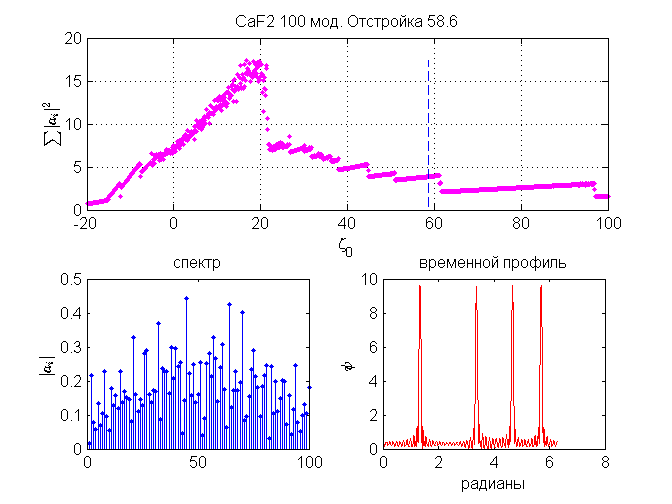
\includegraphics[width = 1\textwidth,height=0.5\textheight]{caf2_main}
 % 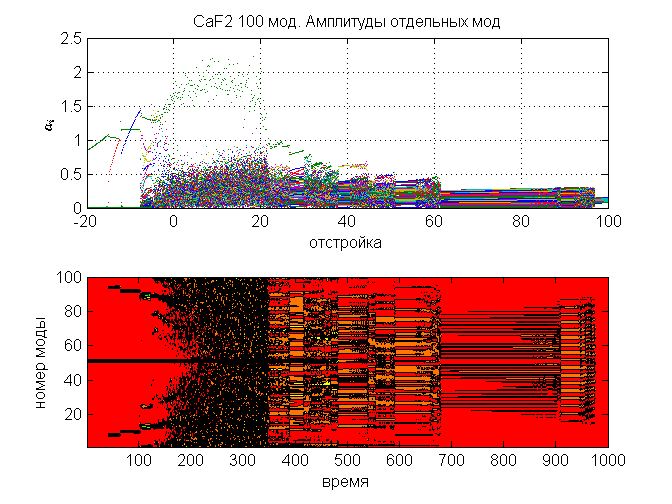
\includegraphics[width = 1\textwidth,height=0.5\textheight]{caf2_modes}
  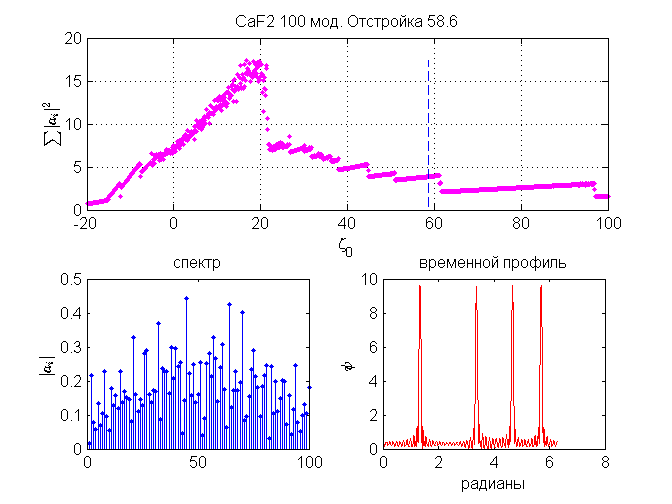
\includegraphics[width = 0.5\textwidth]{caf2_main}
  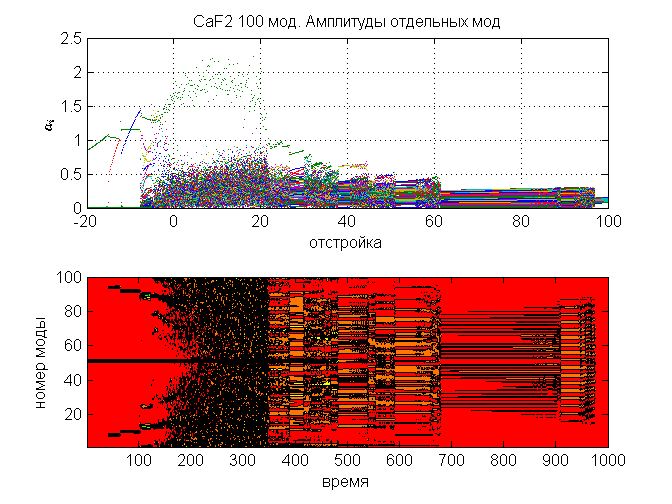
\includegraphics[width = 0.5\textwidth]{caf2_modes}
  \caption{Моделирование 100 мод. Резонатор $CaF_2$. Генерация гребенки в широком диапазоне перестройки лазера} \label{caf2}
\end{figure}

Рассмотрим параметры резонатора, в котором наблюдалась частотная гребенка шириной больше октавы. Рис. \ref{sio2} получен по результатам моделирования для резонатора из $SiO_2$ с параметрами из статьи \cite{DelHaye2011} :
$
Q_0=Q_c=2.7\times10^8,\quad
P_0=2.5\text{ Вт},\quad
\lambda_0=1.56\text{ мкм}, \quad
n_0=1.44,\quad
V_0=5\times10^{-13}\text{ м}^3,\quad
n_2=2.2\times10^{-20}\frac{\text{м}^2}{\text{Вт}},\quad
D_2=10\times10^6\text{ Гц},\quad
D_3=0.$

Резонатор отличается большим $D_2$, мощностью накачки и ОСД. На рисунках видна генерация гребенки в узком диапазоне перестройки лазера. Из-за большой ОСД 200 мод уже покрывают октаву. Результаты моделирования согласуются с выводами авторов статьи.

\begin{figure}
%  \centering
%  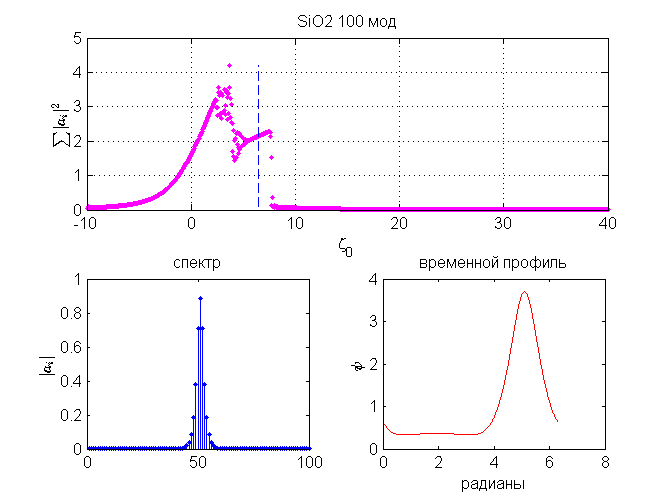
\includegraphics[width = 1\textwidth,height=0.5\textheight]{sio2_100}
 % 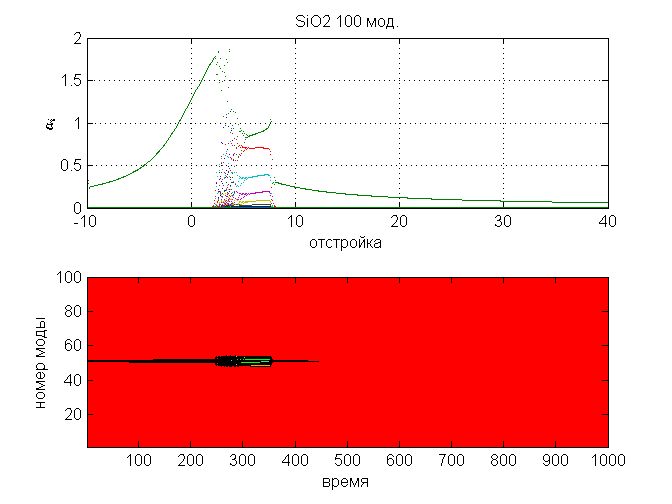
\includegraphics[width = 1\textwidth,height=0.5\textheight]{sio2_100_modal}
  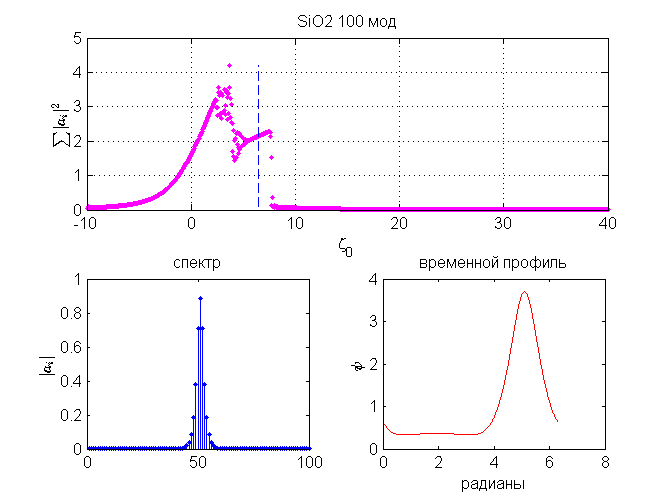
\includegraphics[width = 0.5\textwidth]{sio2_100}
  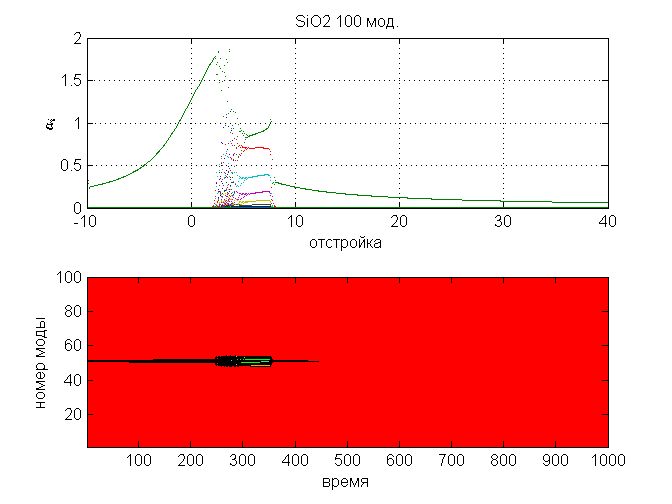
\includegraphics[width = 0.5\textwidth]{sio2_100_modal}
  \caption{Моделирование 100 мод. Резонатор $SiO_2$} \label{sio2}
\end{figure}

\subsection{Сравнение моделирования разными методами}

Для обоснованного использования методов проведем сравнение моделирования системы связанных уравнений с различной правой частью: прямым вычислением суммы или использованием Фурье преобразования \ref{wabnitz_summation}. Рассмотрим резонатор из $MgF_2$ с параметрами из статьи\cite{Herr2014}, см. пункт \ref{subsection_experiment}. Зададим одинаковые параметры резонатора и области перестройки лазера накачки (от $-15$ до $35$ единиц ширины резонанса, счет для $500$ мод). Полученные результаты приведены на рис. \ref{comparison_sum_ft}. Области и режимы генерации совпадают (на верхних графиках). Видны несовпадения в количестве солитонов ($1$ и $3$ соответственно), это объясняется чувствительностью моделирования к начальным шумам в каждой моде. При повторных симуляциях с одинаковым начальным условием количество солитонов совпадало.
\begin{figure}
  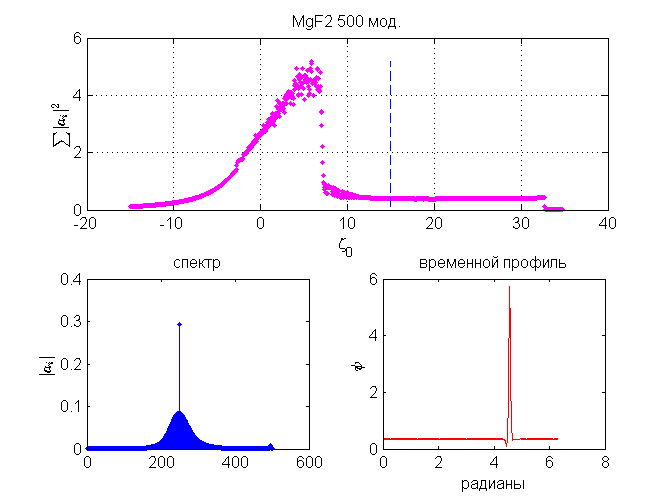
\includegraphics[width = 0.5\textwidth]{mgf2_500cluster}
  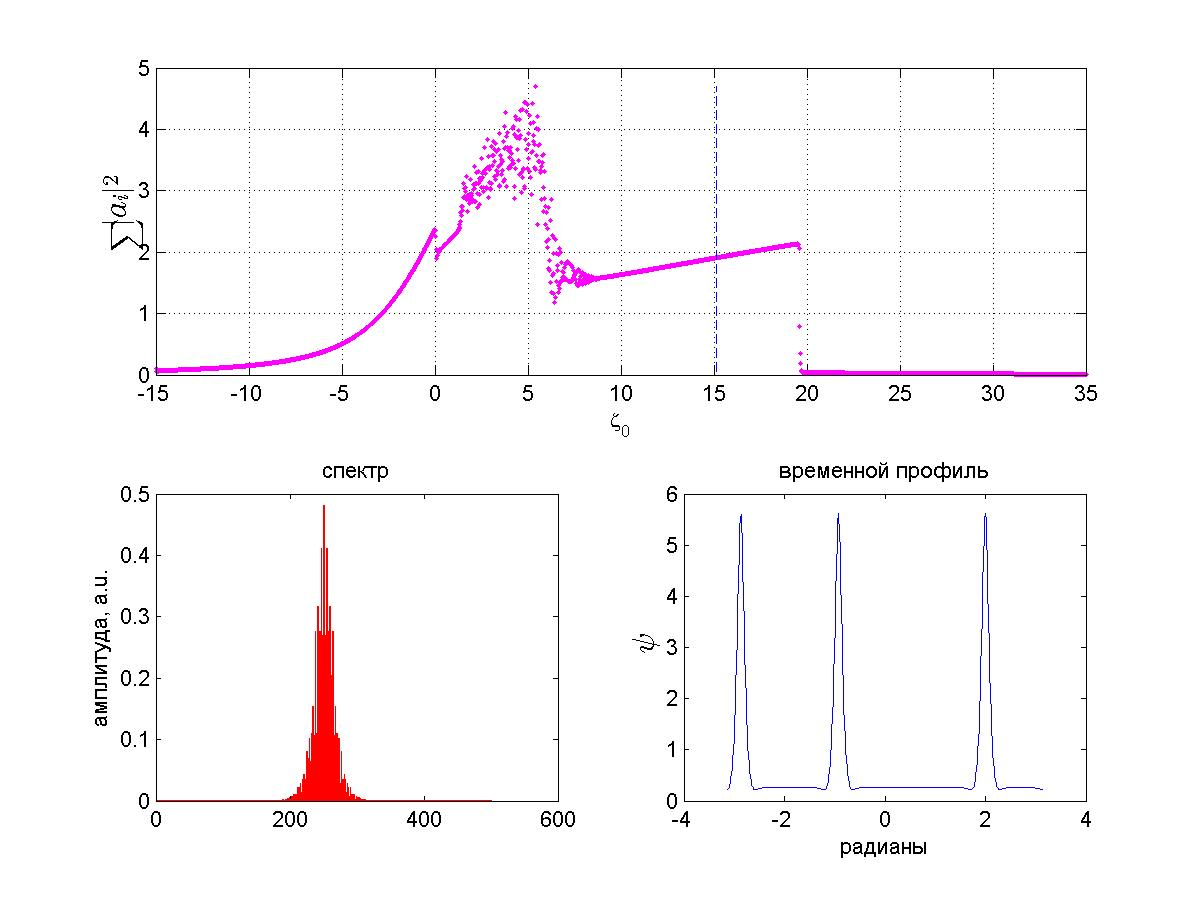
\includegraphics[width = 0.5\textwidth]{mgf2_fft_500}
%  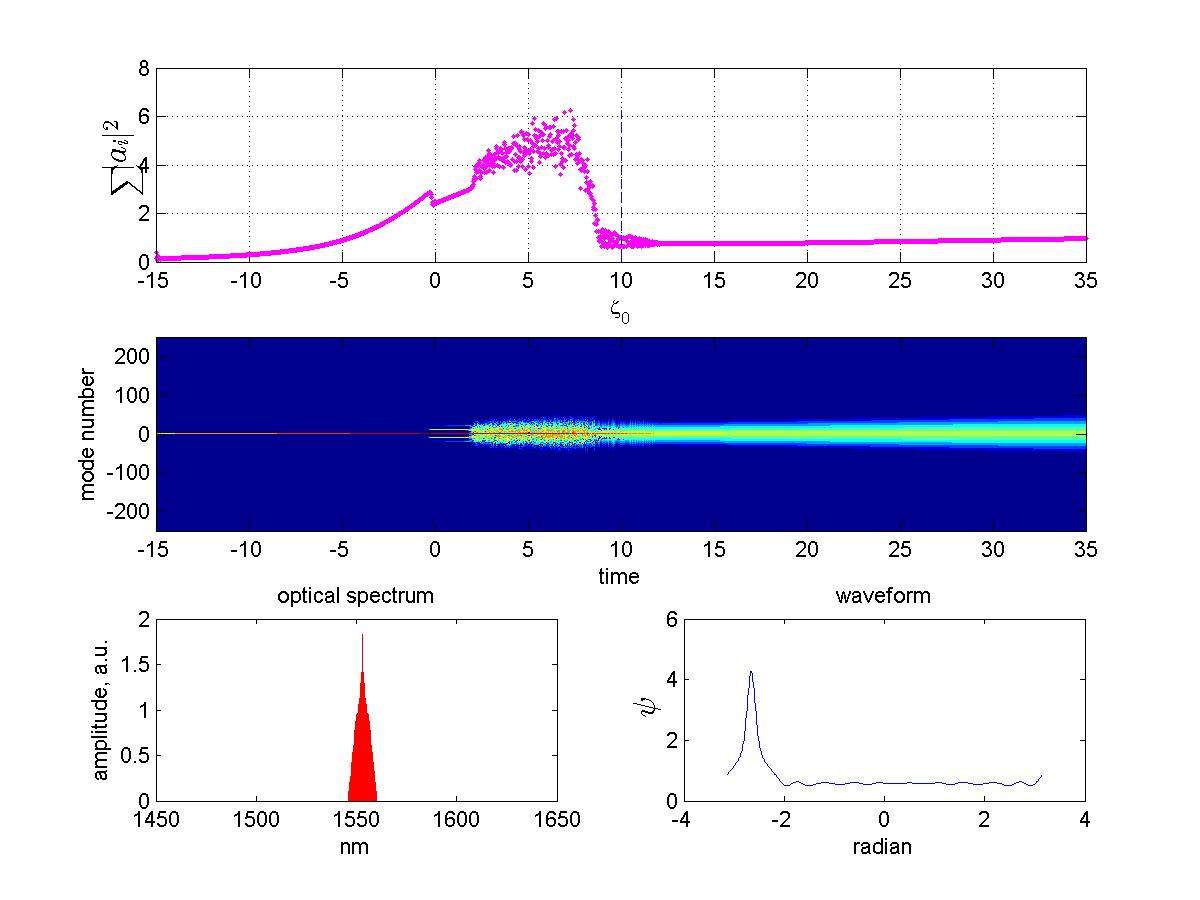
\includegraphics[width = 0.5\textwidth]{mgf2_fft_200}
  \caption{Сравнение методов. Слева счет с прямым суммированием нелинейных членов. Справа с использованием Фурье преобразования. Верхние графики суммы амплитуд мод хорошо совпадают.} \label{comparison_sum_ft}
\end{figure}

Далее сравним результаты моделирования уравнения Луджиато-Лефевера \eqref{LLE} и связанных уравнений в спектральном представлении \eqref{compute_eq}. Зададим одинаковые параметры
$
Q_0=Q_c=5\times10^8,\quad
P_0=100\text{ мВт},\quad
\lambda_0=1.553\text{ мкм},\quad
\omega_0=1.213\times10^{15}\text{ Гц},\quad
n_0=1.376,\quad
V_0=5.6\times10^{-13}\text{ м}^3,\quad
\kappa=\frac{\omega}{Q_0}=1.2\times10^6\text{ Гц},\quad
n_2=0.9\times10^{-20},\quad
g=6.1\times10^{-4},\quad
D_1=2.21\times10^{11}\text{ Гц},\quad
D_2=6.28\times10^4\text{ Гц},\quad
D_3=0\text{ Гц},\quad
\kappa=1.2\times10^6\text{ Гц}.\quad
$
Будем перестраивать лазер накачки от $-15$ до $35$ единиц. Начальным условием в каждой моде выступает нормально распределенный шум $\mathcal{N}(0,1)$. Результаты показаны на рис. \ref{comparison_coupled_lle}. Картина моделирования методом SSFM хорошо совпадает с картиной для связанных уравнений - последовательно наблюдаются рост только моды накачки, зона модуляционной нестабильности, далее стабильная генерация нескольких импульсов. Основные отличия - количество наблюдаемых импульсов и величина отстройки, при которой частотная гребенка пропадает. При повторных симуляциях при других параметрах число импульсов иногда совпадало. Можно утверждать, что обе математические модели дают хорошее совпадение при описании физического явления генерации частотных гребенок в микрорезонаторах.

\begin{figure}
  %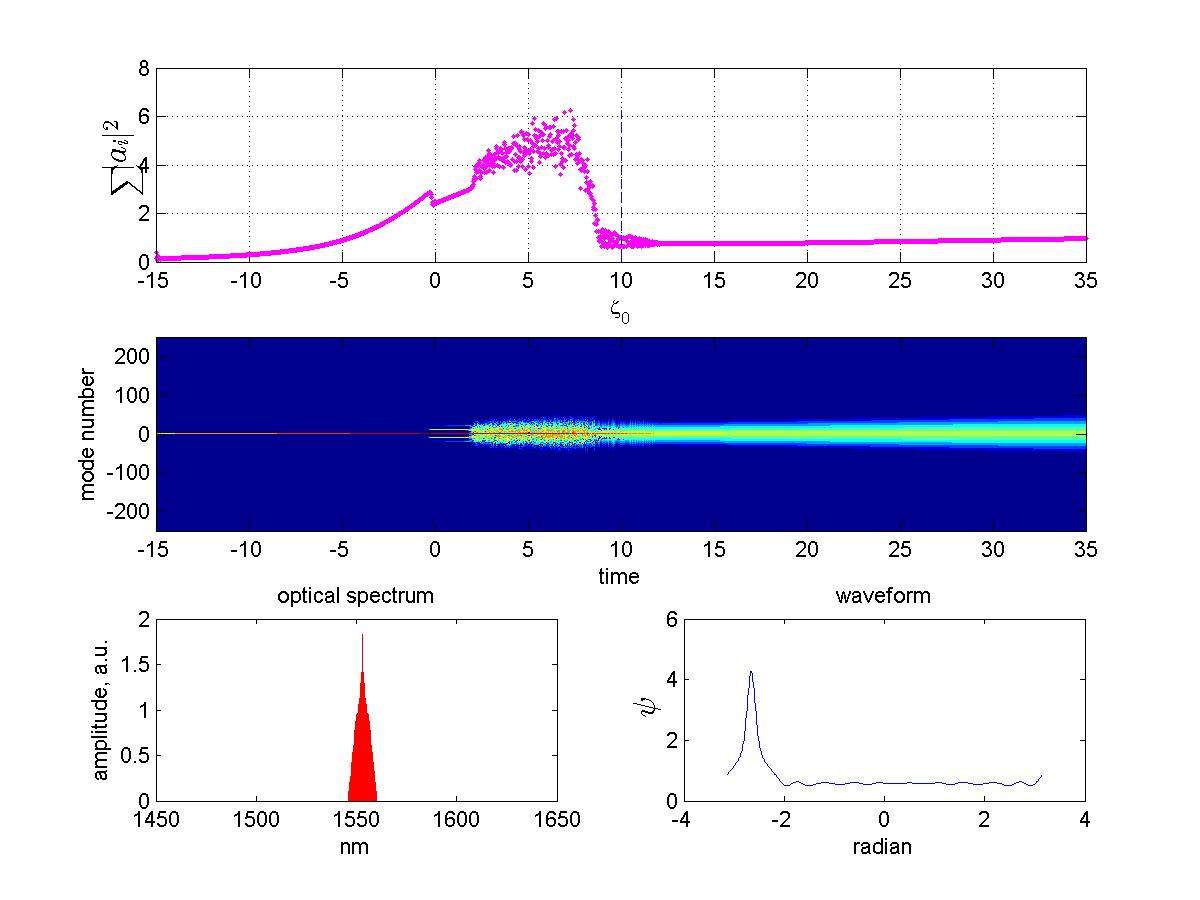
\includegraphics[width = 0.5\textwidth]{mgf2_fft_200}
  %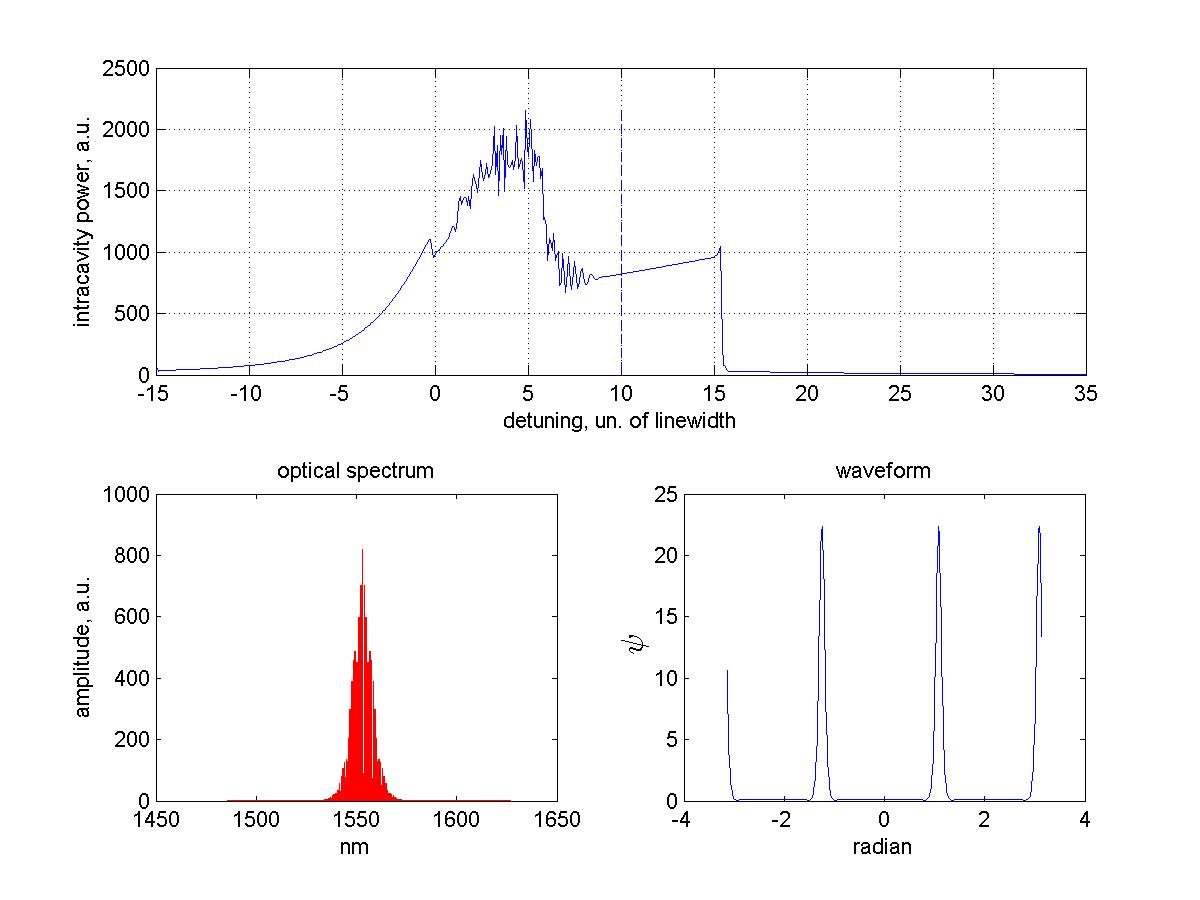
\includegraphics[width = 0.5\textwidth]{mgf2_lle_501}
  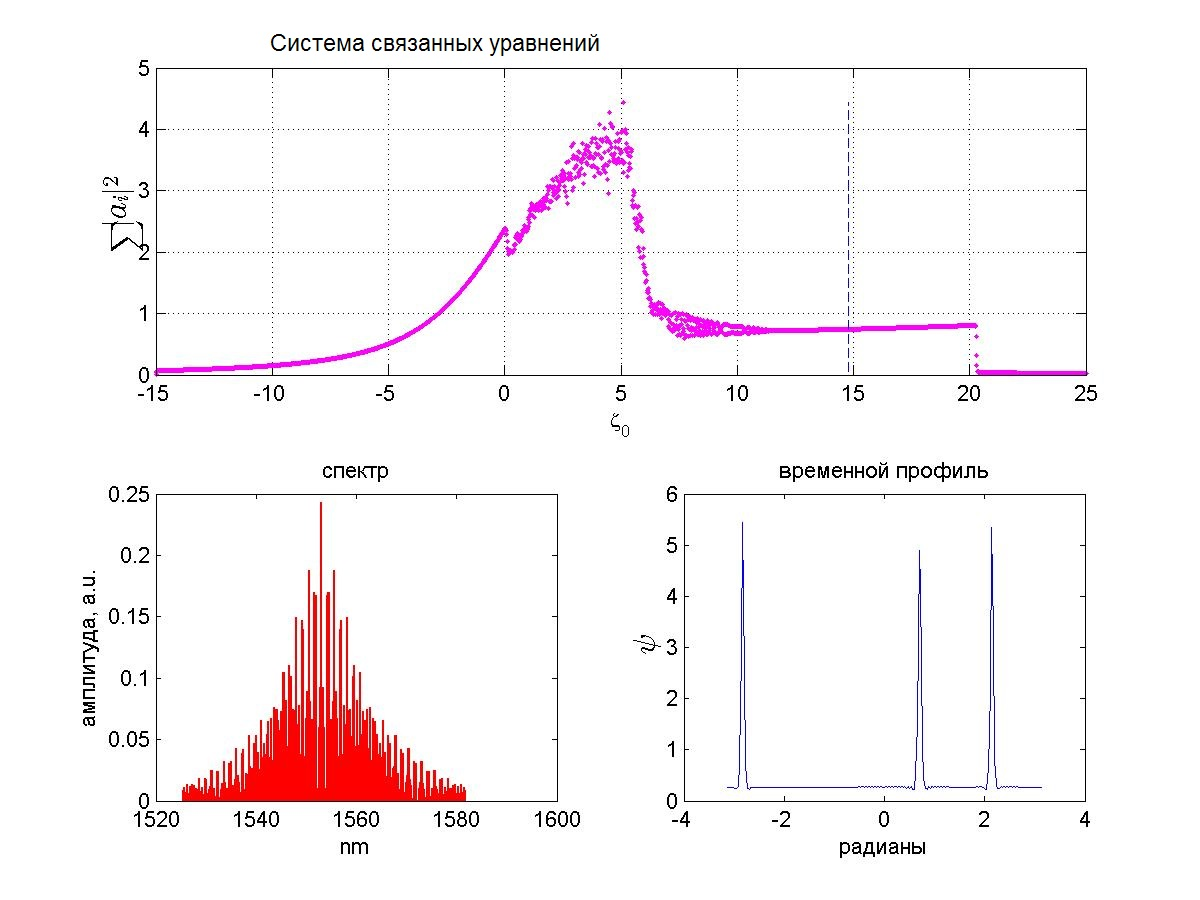
\includegraphics[width = 0.5\textwidth]{mgf2_compare_coupled}
  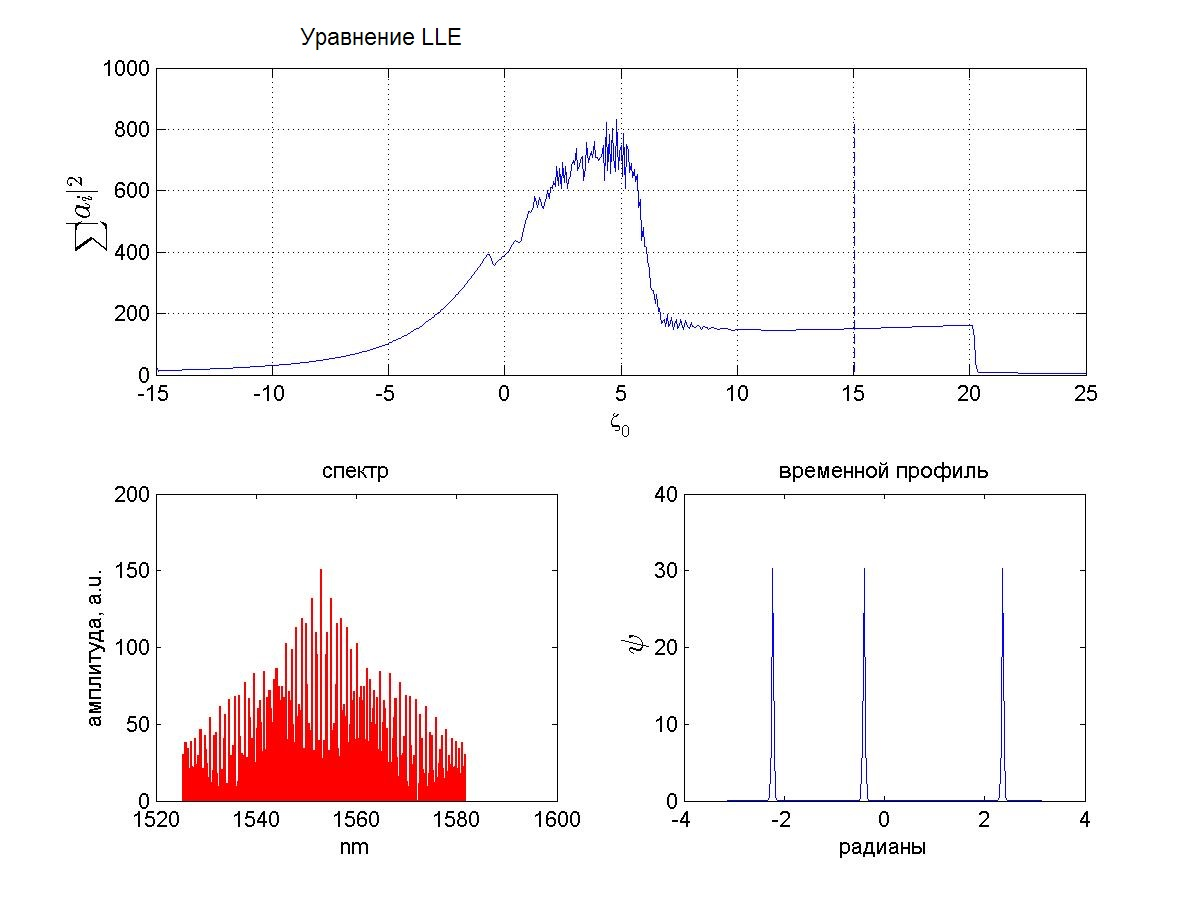
\includegraphics[width = 0.5\textwidth]{mgf2_compare_lle}
  \caption{Сравнение мат. моделей. Слева счет для системы связанных уравнений. Справа для уравнения Луджиато-Лефевера.} \label{comparison_coupled_lle}
\end{figure}

\subsection{Учет нагрева резонатора.}

Для более точного совпадения численного моделирования с экспериментом требуется учет нагрева резонатора лазером накачки, что приводит к другой конфигурации мод и нарушению режима генерации гребенок. К основной системе уравнений \eqref{compute_eq} добавляется уравнение теплопроводности. Следуя \cite{Gorodetsky} получим систему:
\begin{equation}
\frac{\partial a_\mu}{\partial \tau}=-[1+i\zeta_{\mu}-i\Theta]a_\mu+i\sum_{\mu^\prime\le\mu^{\prime\prime}} (2-\delta_{\mu^\prime\mu^{\prime\prime}})a_{\mu^\prime}a_{\mu^{\prime\prime}}a_{\mu^\prime+\mu^{\prime\prime}-\mu}^*+\delta_{0\mu}F,
\end{equation}
\begin{equation}
\frac{\partial \Theta}{\partial \tau}+\frac{2\delta_\theta}{\kappa}\Theta=\frac{n_{2\theta}}{n_2}\frac{2\delta_\theta}{\kappa}\sum_\mu |a_\mu|^2,
\end{equation}
где $\Theta$ - усредненная по объему моды температура.

Выбранная модель предполагает, что сдвиг каждой моды при учете тепловой нелинейности одинаков. Программа была доработана, в связанные уравнения добавлена зависимость отстройки от $\Theta$, вычисление $\Theta$ производилось на каждом шаге по времени. Выбрано отношение $\frac{2\delta_\theta}{\kappa}=20$.  Рис. \ref{therm} дает результат моделирования с учетом небольшого теплового коэффициента $n_{2\theta}=10$, остальные параметры резонатора $MgF_2$ были приведены в предыдущих пунктах.

Был применен новый сценарий - лазер перестраивался от $-15$ до $50$ единиц и далее оставался на отстройке $50$ до конца симуляции. Видно, что генерация гребенки сохраняется, но диапазон требуемой перестройки лазера заметно увеличивается. При численном моделировании удается зафиксировать многосолитонный режим. Однако во всех реальных экспериментах для фиксации такого режима используются различные механизмы тепловой стабилизации.

\begin{figure}
  %\centering
  %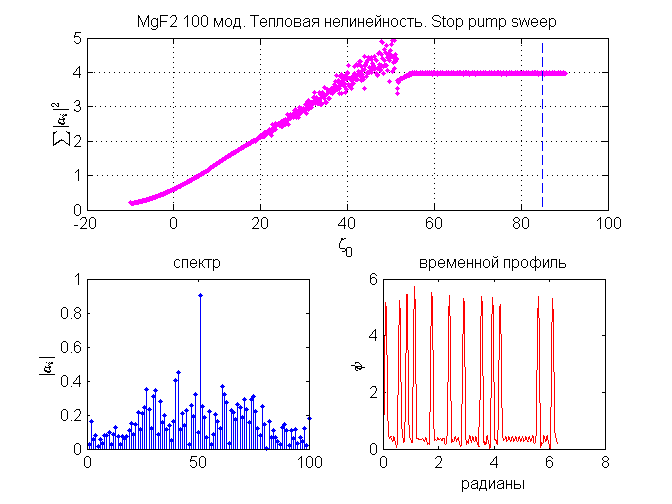
\includegraphics[width = 1\textwidth,height=0.5\textheight]{mgf2_therm_stop_detune}
  %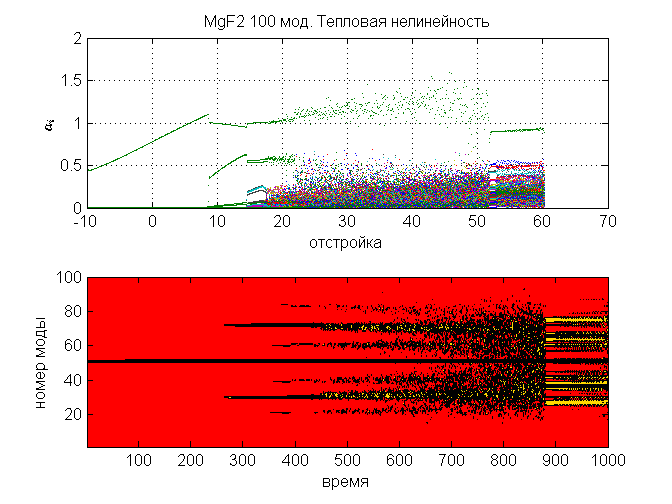
\includegraphics[width = 1\textwidth,height=0.5\textheight]{mgf2_therm_good_modes}
  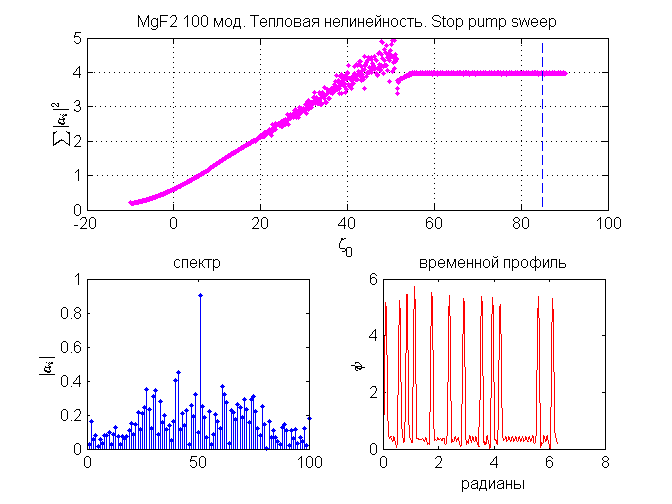
\includegraphics[width = 0.5\textwidth]{mgf2_therm_stop_detune}
  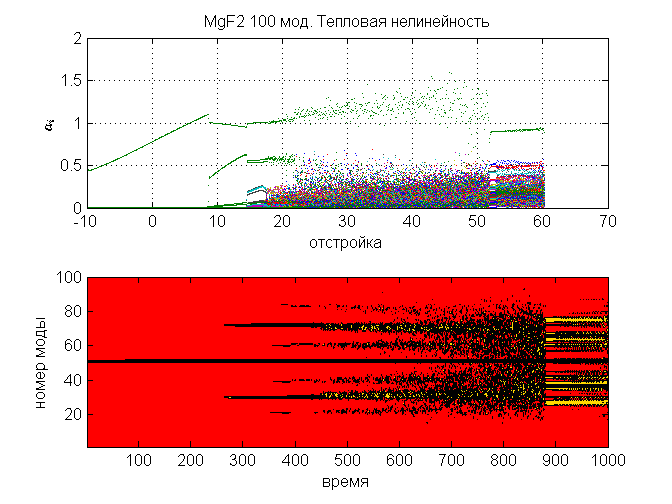
\includegraphics[width = 0.5\textwidth]{mgf2_therm_good_modes}
  \caption{Резонатор из $MgF_2$. Слабая тепловая нелинейность. Фиксация многосолитонного режима происходит при остановке перестройки лазера накачки на $50$} \label{therm}
\end{figure}

\subsection{Отсутствие генерации гребенки.}
Не во всех лабораториях удавалось экспериментально наблюдать солитонный режим. В некоторых случаях возбужденными оказывались лишь небольшое число боковых мод. Приведем сценарии, когда частотная гребенка не наблюдалась и при численном моделировании.

На рис. \ref{no_comb} вверху показан результат для резонатора из $MgF_2$ при большой тепловой нелинейности $n_{2\theta}=100$. Боковые моды не возбуждаются в широком диапазоне перестройки (проводилась симуляция от $-20$ до $100$ единиц).

На рис. \ref{no_comb} внизу показан сценарий одновременной перестройки и линейного увеличения мощности накачки от 0 до $P_0=100$ мВт. Боковые моды не возбуждались.

Был рассмотрен сценарий, когда лазер отстроен на фиксированную величину $10$, его мощность линейно увеличивается от 0 до $P_0=100$ мВт. Оптическая гребенка в этом случае не наблюдалась.

Гребенка также не наблюдалась при малых значениях добротности $Q\approx10^5$ или больших значениях $D_2\approx10^7$ Гц.

\begin{figure}
  %\centering
  %  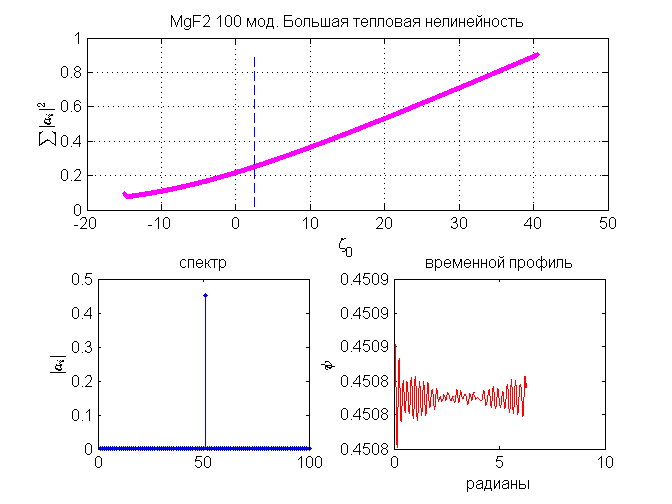
\includegraphics[width = 1\textwidth,height=0.5\textheight]{mgf2_big_therm}
 % 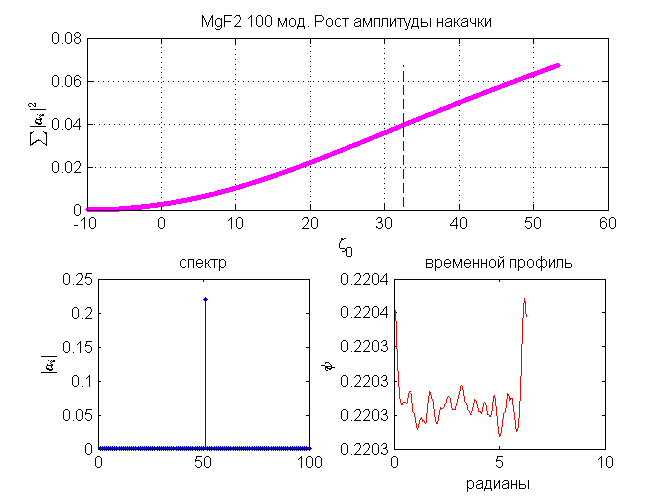
\includegraphics[width = 1\textwidth,height=0.5\textheight]{mgf2_f_grow_therm}
  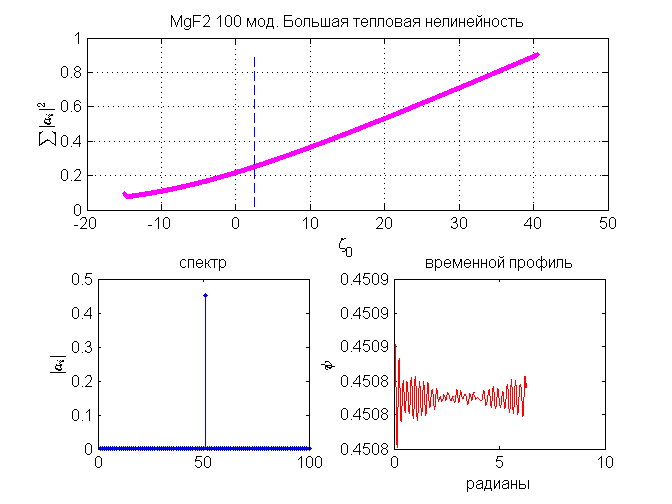
\includegraphics[width = 0.5\textwidth]{mgf2_big_therm}
  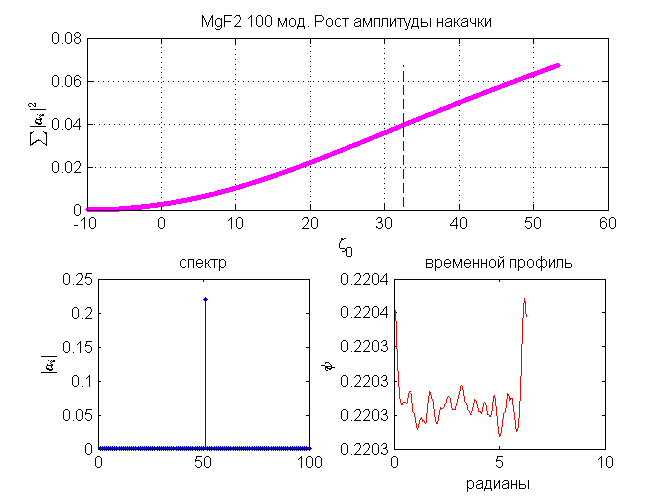
\includegraphics[width = 0.5\textwidth]{mgf2_f_grow_therm}
  \caption{Отсутствие гребенки. Резонатор из $MgF_2$. Большая тепловая нелинейность (слева). Рост мощности накачки (справа)} \label{no_comb}
\end{figure}

\subsection{Различные сценарии моделирования}

Для резонатора из $MgF_2$ моделировались сценарии фиксации солитонного режима. Рис. \ref{step_detune} дает зависимости: а) лазер равномерно перестраивается и останавливается на отстройке, соответствующей солитонному режиму; б) лазер перестраивается скачком с отстройки, соответствующей хаотическому режиму, на отстройку, соответствующую солитонному режиму (режим рассмотрен в \cite{Matsko2013}). В обоих случаях симуляция давала желаемый результат - фиксацию солитонного режима. Однако в эксперименте этому препятствует большая тепловая нелинейность.

\begin{figure}
%  \centering
%  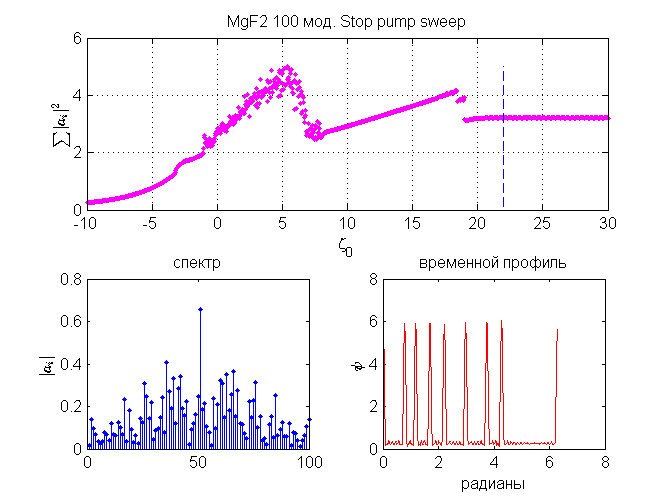
\includegraphics[width = 1\textwidth,height=0.5\textheight]{mgf2_stop_pump_sweep}
 % 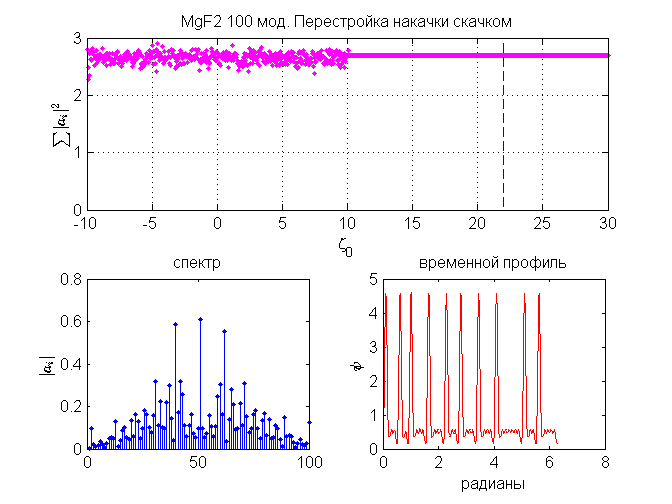
\includegraphics[width = 1\textwidth,height=0.5\textheight]{step_detune_main}
  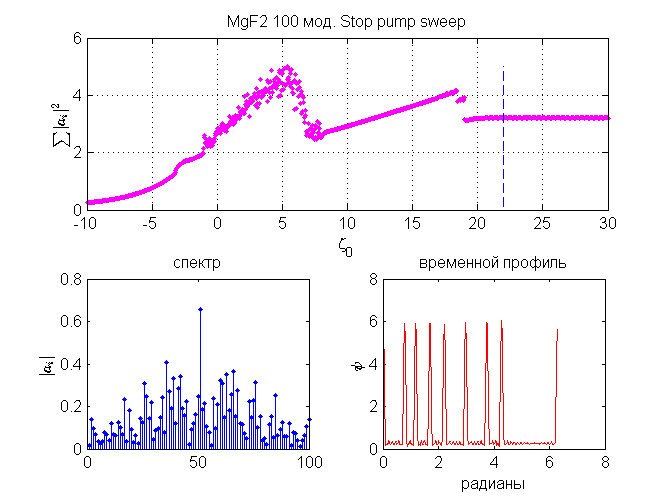
\includegraphics[width = 0.5\textwidth]{mgf2_stop_pump_sweep}
  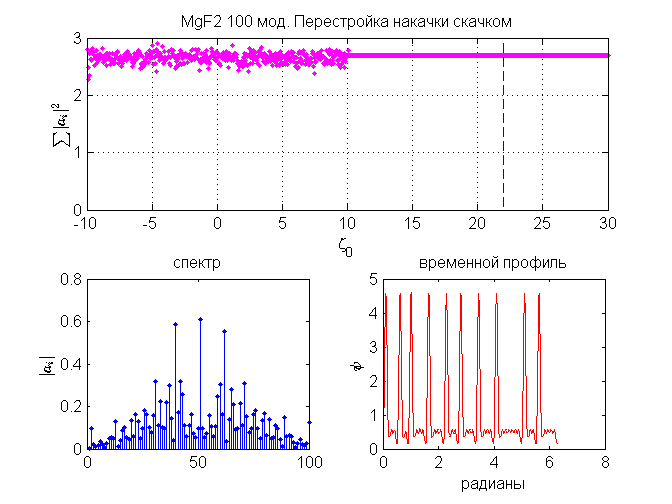
\includegraphics[width = 0.5\textwidth]{step_detune_main}
  \caption{Фиксация солитонного режима. Остановка перестройки лазера накачки (слева). Перестройка скачком (справа)} \label{step_detune}
\end{figure}

С экспериментальной точки зрения интересен сценарий сдвига собственной частоты моды накачки на постоянную величину от соседних мод. Рисунок \ref{pump_shift} показывает динамику гребенки в зависимости от сдвига центральной частоты моды накачки. Тем самым моделируется отклонение от разложения $\omega_\mu=\omega_0+D_1\mu+\frac{1}{2}D_2\mu^2$ в нулевой точке. Сдвиг выражен в единицах ширины резонансной кривой. При больших сдвигах в положительную или отрицательную сторону гребенка не генерируется (при сохранении аномальной дисперсии).

\begin{figure}
  \centering
  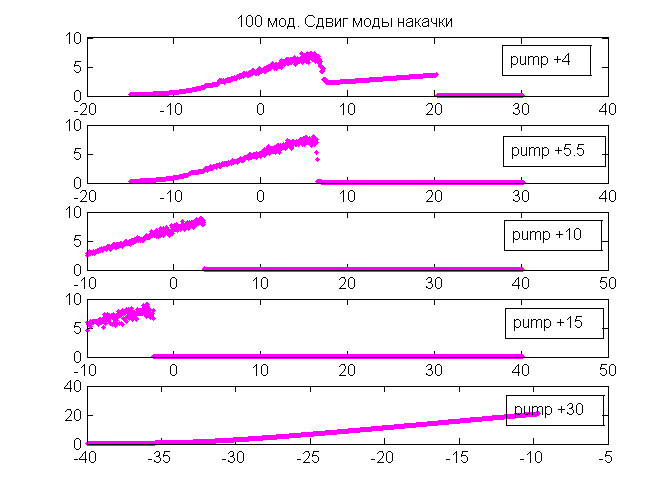
\includegraphics[width = 1\textwidth,height=0.5\textheight]{pump_shift_plus}
  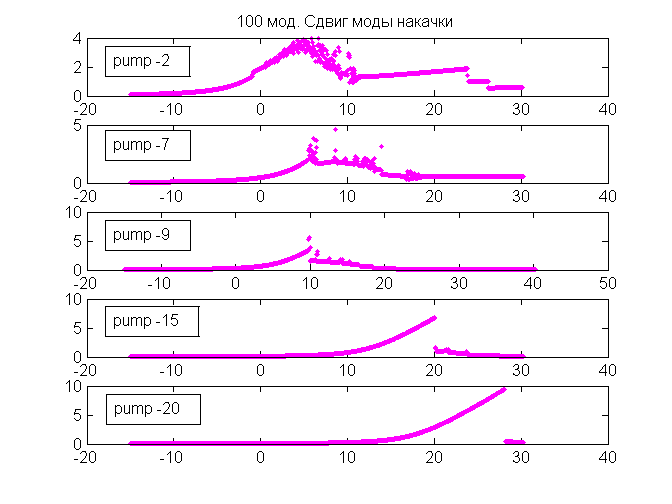
\includegraphics[width = 1\textwidth,height=0.5\textheight]{pump_shift_minus}
  \caption{Измененный закон дисперсии: сдвиг частоты моды накачки в единицах ширины резонансной кривой} \label{pump_shift}
\end{figure}

Другим интересным для эксперимента параметром является фазовая модуляция лазера накачки. В спектральном представлении фазовая модуляция эквивалентна возбуждению боковых мод. В программу были внесены изменения -  помимо центральной моды подавалась постоянная накачка разного знака в $2$ соседние моды. Рис. \ref{phase_pump} показывает результат моделирования - генерация гребенки сохраняется, на графике амплитуд отдельных мод видна их осциллирующая форма. Однако при увеличении накачки в боковые моды (соответственно глубины фазовой модуляции) пропадают области многосолитонного режима.

\begin{figure}
%  \centering
%  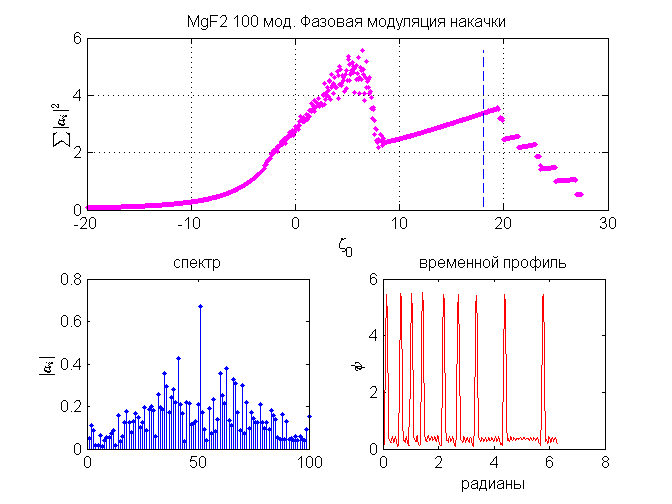
\includegraphics[width = 1\textwidth,height=0.5\textheight]{phase_pump}
 % 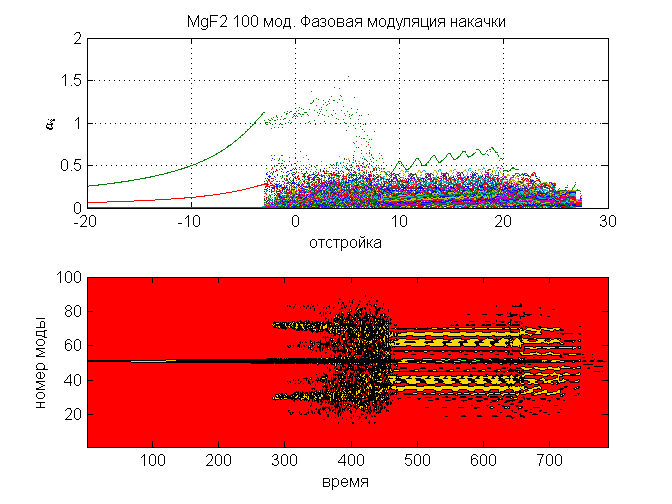
\includegraphics[width = 1\textwidth,height=0.5\textheight]{phase_pump_modal}
  \includegraphics[width = 0.5\textwidth]{phase_pump}
  \includegraphics[width = 0.5\textwidth]{phase_pump_modal}
  \caption{Фазовая модуляция накачки} \label{phase_pump}
\end{figure}

\subsection{Влияние дисперсии резонатора}

В экспериментальных работах исследуется влияние дисперсии высоких порядков на формирование частотной гребенки. Рассмотрим разложение $\omega_\mu=\omega_0+D_1\mu+\frac{1}{2}D_2\mu^2+\frac{1}{6}D_3\mu^3$. Дисперсия второго порядка $D_2=-\frac{c}{n}D_1^2\beta_2$, где $\beta_2$ - дисперсия групповой скорости. Положительная $D_2$ соответствует аномальной дисперсии резонатора и параболическому отличию распределения мод от эквидистантности. Коэффициенты $D_2, D_3$ оцениваются аналитически или численно, учитывая материальную и геометрическую дисперсии. Для резонатора из $MgF_2$ проведем моделирование для разных значений этих параметров. Результаты представлены на рис. \ref{d2d3_plot}. Цветом дано отношение пиковой и средней мощности внутри резонатора. Оно выступает как индикатор количества солитонов, максимальное значение соответствует односолитонному режиму. Картина симметрична для положительных и отрицательных $D_3$. Минимальное число солитонов достигается при устремлении $D_3\rightarrow 0$ и небольших $D_2\ge0$.

\begin{figure}
  \centering
  \includegraphics[scale = 0.5]{d2d340p40}
  \caption{Резонатор из $MgF_2$. Зависимость числа генерируемых солитонов от дисперсии второго и третьего порядка. Цветовая шкала показывает отношение пиковой и средней мощности внутри резонатора. Максимальное значение (красный цвет) соответствует односолитонному режиму. Меньшие значения (синий цвет) соответствуют многосолитонным режимам и режимам без генерации солитонов.} \label{d2d3_plot}
\end{figure}

Далее было выполнено моделирование отклонения от параболического вида $\omega_\mu-\omega_0-D_1\mu=\frac{1}{2}D_2\mu^2$ путем добавления случайного шума в каждую моду с нормальным распределением. Случайная величина с гауссовским распределением $\mathcal{N}(0,1)$ получалась из случайных величин с равномерным распределением по алгоритму Box-Muller \cite{Press2002}. На рис. \ref{gaus} приведены графики динамики гребенки при заданном распределении мод по частоте (отклонению от эквидистантности). Увеличивая дисперсию шума, мы сужаем области многосолитонного режима. Однако последний график показывает, что даже при значительных отклонениях от параболического вида для удаленных мод, но при сохранении такового для близких к центральной моде накачки, хорошо наблюдается гребенка с солитонными режимами.

\begin{figure}
  \centering
%  \includegraphics[width = 1\textwidth,height=0.5\textheight]{gaus1}
  \includegraphics[width = 1\textwidth,height=0.5\textheight]{gaus2}
  \caption{Отклонение от параболического разложения \eqref{dispersion_eq} для мод. Цветовая шкала показывает отношение пиковой и средней мощности внутри резонатора. Максимальное значение (красный цвет) соответствует односолитонному режиму. Меньшие значения (синий цвет) соответствуют многосолитонным режимам и режимам без генерации солитонов.} \label{gaus}
\end{figure}

Известно, что связь между семействами мод в резонаторе дополнительно изменяет собственные частоты и может приводить к особой картине пересечения мод \cite{HerrPRL2014}. В упрощенной модели эффект нормального расщепления мод может быть параметризован как гиперболическое отличие распределения мод $\omega_\mu=\omega_0+D_1\mu+\frac{1}{2}D_2\mu^2+\frac{a/2}{\mu-b-0.5}$, где $a$ показывает на сколько выбивается мода с номером $b$. Результат моделирования для различных $a,b$ приведен на рис. \ref{offsetplot}. Картина центрально-симметричная, видно, что даже небольшие выбивания близких к центральной мод приводят к картине без солитонов. Этот результат согласуется с ранними экспериментальными данными \cite{HerrPRL2014}. Однако позже мною экспериментально неоднократно замечалось, что наличие расщепления моды накачки, приводит к уширению солитонной ступеньки. При дальнейшей настройке на солитонный режим, наблюдалось большое число дисперсионных волн на эффектах нормального расщепления мод, сигнал биений на частоте повторения солитона был шумным (порядка 10 кГц). Иногда наблюдалась одновременная параметрическая генерация отдельных линий на другом семействе мод, т.ч. фактически один лазер генерировал гребенки на двух семействах мод при накачке в месте их пересечения.

\begin{figure}
  \centering
  \includegraphics[width = 0.8\textwidth]{offsetplot}

  \includegraphics[width = 0.2\textwidth]{mode_crossing}
%  \includegraphics[scale = 0.5]{offsetplot}
 % \includegraphics[width = 0.3\textwidth]{mode_crossing}
  \caption{Резонатор из $MgF_2$. Гиперболическое отличие частот в законе дисперсии. Параметр $a$ показывает на сколько выбивается мода с номером $b$. Цветовая шкала дает отношение пиковой и средней мощности внутри резонатора. Максимальное значение соответствует односолитонному режиму} \label{offsetplot}
\end{figure}

\subsection{Моделирование генерации дисперсионной волны по экспериментальным данным}

В эксперименте \cite{Brasch2016} впервые экспериментально продемонстрирован оптический временной солитон и индуцированная им дисперсионная волна в интегральном микрорезонаторе из $Si_3N_4$ \ref{brashch_dispersive_wave}. При наличии дисперсии высоких порядков оптический солитон может излучать дисперсионную волну \cite{PhysRevA.51.2602} вблизи частот с нулевой суммарной дисперсией. Хотя в волоконной оптике этот эффект считается вредным для некоторых приложений, для микрорезонаторов он позволил расширить спектральное покрытие гребенки и при правильном выборе геометрии резонатора дает мощные пики по краям спектра, необходимые при удвоении частоты для самосинхронизации f-2f \cite{Spencer2018}. При наличии дисперсии третьего и более высоких порядков спектр возмущенного солитона перестает быть симметричным, максимум спектра сдвигается и возникает дополнительный мощный спектральный пик. Во временном представлении солитон имеет осциллирующий хвост (отсюда другое название по аналогии: оптическое черенковское излучение). Положение спектрального пика определяется из условия нуля суммарной дисперсии: $\mu_{dw}=\frac{-3D_2}{D_3}$ при $D_4=0$ и $\mu_{dw}=\frac{-2D_3}{D_4}\pm\sqrt{(\frac{2D_3}{D_4})^2-\frac{12D_2}{D_4}}$ при $D_4\neq0$.

Было проведено численное моделирование по параметрам, полученным из экспериментальных данных по измерению дисперсии в диапазоне вблизи накачки ($D_3,D_4$ подбирались вручную): $D_2/2\pi=2.2$ МГц, $D_3/2\pi=25$ кГц, $D_4/2\pi=-300$ Гц. Мощность накачки 1 Вт, добротность $Q=10^6$. Начальным условием являлся односолитонный режим, полученный из набора предыдущих симуляций. Эффективная отстройка составила $\zeta=12$ для наилучшего совпадения с экспериментом.  Вычисленное значение $\mu_{dw}=-200$, что близко к экспериментальному значению -195. На рис. \ref{brashch_dispersive_wave} зеленым показана огибающая спектра, полученная при моделировании, видно хорошее совпадение по мощности линий, но с общим сдвигом. Отсутствие в эксперименте сдвига максимума огибающей спектра связано с тем, что в нитриде кремния одновременно происходит сдвиг спектрального максимума в противоположную сторону из-за эффекта Рамана \cite{Karpov2016}, а также из-за не учитываемой в моделировании зависимости нелинейного коэффициента $\gamma$ от частоты.

\begin{figure}
  \centering
  \includegraphics[width = 0.9\textwidth]{brashch_dispersive_wave}

  \caption{А: оптический временной солитон и индуцированная им дисперсионная волна в интегральном микрорезонаторе из $Si_3N_4$, зеленым дана огибающая гребенки из численного моделирования по параметрам из эксперимента; В: дисперсионная кривая микрорезонатора, вычисленная методом FEM моделирования с нанесенными экспериментальными точками.} \label{brashch_dispersive_wave}
\end{figure}


\subsection{Моделирование уравнения Луджиато-Лефевера методом конечных разностей}

Моделирование уравнения LLE \eqref{LLE} c начальным профилем
\begin{equation} \label{initial_cond_soliton}
\psi(0,\theta)=\sqrt{2\zeta_0}\exp (i \arccos(\frac{\sqrt{8\zeta_0}}{\pi f}))\sum_j sech(\sqrt{\frac{\zeta_0}{d_2}}(\theta-\theta_j))
\end{equation}
было проведено в пакете Mathematica. Использовалась функция NDSolve, которая реализует конечно-разностный метод. Для одного солитона методом проб и ошибок были найдены границы изменений параметров $\zeta_0,f$, при которых солитон распространяется без изменения профиля.
%(представлены на рис. \ref{nls}).

Для многосолитонных профилей удалось проследить, как, изменяя ширину и расстояние между солитонами, удается добиться распространения без столкновений за длительное время (рис. \ref{2solitons},\ref{3solitons})
\begin{figure}
  \includegraphics[width = 0.5\textwidth,height=0.25\textheight]{2solitons_gap1}
  \includegraphics[width = 0.5\textwidth,height=0.25\textheight]{2solitons_gap2}
\end{figure}

\begin{figure}
  \includegraphics[width = 0.5\textwidth,height=0.25\textheight]{2solitons_gap4}
  \includegraphics[width = 0.5\textwidth,height=0.25\textheight]{2solitons_gap6}
  \caption{Столкновение двух солитонов. Увеличивая начальное расстояние между солитонами, можно добиться отсутствия столкновения.} \label{2solitons}
\end{figure}

\begin{figure}

  \includegraphics[width = 0.5\textwidth]{3solitons_gap6}
  \includegraphics[width = 0.5\textwidth]{3solitons_gap12}
  \caption{Столкновение трех солитонов. Увеличивая начальное расстояние между солитонами, можно добиться отсутствия столкновения.} \label{3solitons}
\end{figure}


\section{Моделирование возбуждения оптических частотных гребенок и платиконов в микрорезонаторах с нормальной дисперсией групповой скорости}

Достичь в микрорезонаторах аномальной суммарной дисперсии групповой скорости (ДГС) в широкой полосе частот для произвольной центральной частоты сложно, т.к. материальная ДГС в видимом и ближнем ИК диапазонах в основном нормальная и большая по модулю, т.ч. компенсировать ее подбором геометрии резонатора нельзя. Поэтому необходимо найти пути генерации оптических частотных гребенок при нормальной дисперсии.

Известно, что в реальных микрорезонаторах наблюдаемые дисперсионные соотношения могут существенно отличаться от теоретических, например, из-за наличия связи между различными семействами мод. В частности, это может приводить к существенному сдвигу резонансных частот. Благодаря этому закон дисперсии вблизи “сдвинутой” моды может характеризоваться наличием локальной эффективной аномальной дисперсии, что в свою очередь является причиной появления модуляционной неустойчивости, приводящей к дальнейшему возбуждению частотной гребенки с светлыми или темными солитонами.

С помощью численного моделирования было показано, что если сдвинута накачиваемая лазером мода резонатора, либо из-за эффекта нормального расщепления мод, либо в результате сильного эффекта затягивания, то возможна генерация стабильных ультракоротких импульсов с плоской вершиной, которые назовем платиконами. Будет показано, что если такое выбивание моды достаточно большое (величиной в несколько ширин линий моды резонатора), тогда платиконы могут быть сгенерированы спонтанно, когда лазер перестраивается через эффективную нулевую отстройку высокодобротного резонанса. Длительность таких сгенерированных импульсов можно непрерывно менять, изменяя отстройку лазера накачки от резонанса.

Моделирование было проведено для системы связанных уравнений:
%
\begin{equation}
\frac{\partial a_\mu}{\partial \tau}=-[1+i\zeta_{\mu}]a_\mu+i\sum_{\mu^\prime,\mu^{\prime\prime}} a_{\mu^\prime}a_{\mu^{\prime\prime}}a_{\mu^\prime+\mu^{\prime\prime}-\mu}^*+\delta_{0\mu}f,
\end{equation}

Для анализа использовалось разложение дисперсионного закона в ряд Тэйлора до 2 порядка, дисперсией более высокого порядка не учитывались $\omega_\mu=\tilde\omega_0-\delta_{0\mu}\Delta+D_1\mu+\frac{1}{2}D_2\mu^2$,  где $\tilde\omega_0$ не возмущенная частота моды накачки, $\Delta$ описывает интересующий сдвиг моды накачки и $\delta_{0\mu}$ символ Кронекера. Для нормальной дисперсии $D_2<0$.

Для моделирования использовались следующие параметры MgF$_2$ микрорезонатора: длина волны $\lambda=2\pi c/\omega_0=1.5$ $\mu$m, $n_0=1.37$, $n_2=0.9\times 10^{-20}$ m$^2$/W, $V_{\mathrm{eff}}=5.6\times 10^{-13}$m$^3$,  $Q_0=Q_\text{ext}=4\times 10^8$, $D_2/(2\pi)=-10$kHz. Мощность накачки $P_\mathrm{in}=50$mW соответсвует приблизительно $f\approx 4.11$. Численно было проверено, что качественно похожие результаты получаются и для параметров резонатора из нитрида кремния\cite{Brasch2016}.

Система уравнений решалась численно с помощью адаптивного метода Рунге-Кутта для 501 моды. В качестве начального условия генерировалось слабая шумоподобная затравка (на уровне вакуумных флуктуаций). Для анализа рассчитывалась усредненная интенсивность внутри микрорезонатора $U=\sum_\mu |a_\mu|^2$ и распределение поля $\psi(\phi)=\sum_\mu a_\mu \exp(i\mu\phi)$, где $\phi$ азимутальный угол.

Для моделирования процесса генерации солитонов при перестройке частоты накачки расстройка $\zeta_0$ медленно менялась со временем от отрицательной величины $\zeta_0(0)=-20$, соответствующей отстройке накачки в синюю область, до значительной положительной величины.  При отсутствии или отрицательной величине сдвига моды накачки наблюдался характерная картина треугольного резонанса, соответствующая простому одночастотному решению. Однако при наличии существенного сдвига моды накачки в резонансной характеристике $U(\zeta_0)$ появлялась характерная ступенька, сигнализирующая о переходе в режим генерации импульсов Рис.\ref{platicon_triangles}(а).

\begin{figure}
  \centering
  \includegraphics[width = 1\textwidth,height=0.5\textheight]{triangles}
  \caption{Зависимость усредненной интенсивности внутри микрорезонатора $U$ от нормированной отстройки $\zeta_0$ (a) для различных значений сдвига моды накачки при $f=4.11$ и (в) для различных амплитуд накачки $2\Delta/\kappa=8$} \label{platicon_triangles}
\end{figure}

При остановке перестройки частоты вблизи этой ступеньки солитонный режим сохранялся неограниченное время.
При увеличении мощности накачки “ступенька” становилась более заметной и сдвигалась по частоте к большим значениям расстройки (рис. \ref{platicon_triangles}(б)).

Построенное в таком режиме распределение поля показало наличие локализованных импульсов, обладающих характерным профилем с плоской вершиной (рис. \ref{platicons}(a)]. Заметим, что такие импульсы могут быть также идентифицированы как некие участки, разделяющие два последовательных темных солитона, интервал между которыми равен времени обхода микрорезонатора. В этом смысле можно говорить, как о генерации последовательности темных солитонов, так и о генерации последовательности платиконов. Спектр платиконов обладает двумя ярко выраженными крыльями (рис. \ref{platicons}(b)). Подобные спектры наблюдались в экспериментах по генерации частотных гребенок в интегральных резонаторах с нормальной дисперсией \cite{Huang2015prl}.

\begin{figure}
  \centering
  \includegraphics[width = 1\textwidth,height=0.5\textheight]{platicons}
  \caption{Характерные временные профили поля внутри резонатора (левая панель) и спектры платиконов для различных значений отстройки лазера накачки (правая панель)} \label{platicons}
\end{figure}


На рис. \ref{platicons} хорошо видна особенность платиконов: их длительность и, соответственно, ширина спектра зависят от частоты и, следовательно, могут перестраиваться в широком диапазоне при перестройке частоты. Увеличение частоты накачки (уменьшение отсройки) приводит к уширению импульса и сужению его спектра.

\begin{figure}
  \centering
  \includegraphics[width = 1\textwidth,height=0.5\textheight]{existence}
  \caption{(Левая панель) результаты численного моделирования процесса генерации платиконов для сдвига различных мод. Цветовая гамма показывает отношение пиковой интенсивности к усредненной. Яркая полоса вблизи центральной моды соответствует генерации платиконов, описанных выше. (правая панель) Область существования (синий цвет) и возбуждения платиконов (оранжевый цвет).} \label{platicons_existence}
\end{figure}

Численное моделирование показало, что генерация платиконов наиболее эффективна при сдвиге моды накачки $\mu=0$ (рис. \ref{platicons_existence}(a)). Возбуждение солитонов возможно, если величина сдвига превосходит некое пороговое значение (рис. \ref{platicons_existence}(б)). При достаточном сдвиге моды накачки возбуждение платиконов возможно даже без перестройки частоты, если частота накачки соответствует области мягкого возбуждения.

\begin{figure}
  \centering
  \includegraphics[width = 1\textwidth,height=0.5\textheight]{famdetune}
  \caption{(а) Трансформация дискретного спектра темных солитонов в квазинепрерывный спектр платиконов при увеличении величины сдвига моды накачки. б) Профили различных типов темных солитонов, существующих при одном и том же значении частоты, соответствующем пунктирной линии на левой панели.} \label{platicons_famdetune}
\end{figure}

В отсутствие сдвига возможно существование темных солитонов (похожих на провалы интенсивности на фоне некоторого постоянного уровня), предсказанных ранее. В одном и том же частотном диапазоне может существовать множество типов темных солитонов, отличающихся сложностью профиля (рис. \ref{platicons_famdetune}(б)). Можно сказать, что эти солитоны образуют дискретные энергетические уровни, причем уровни с меньшей энергией, соответствующие более широким провалам, существуют в более узком частотном диапазоне (рис. \ref{platicons_famdetune}(а)). Следовательно, в этом случае перестройка частоты может приводить только к ступенчатому уменьшению ширины провала. При постепенном увеличении величины сдвига моды накачки дискретный спектр преобразуется в квазинепрерывный (рис. \ref{platicons_famdetune}(а)), и именно при такой трансформации спектра становится возможной мягкая генерация платиконов.

\begin{figure}
  \centering
  \includegraphics[width = 1\textwidth,height=0.5\textheight]{famdisp}
  \caption{Зависимости усредненной интенсивности от отстройки лазера накачки (a,в) и профили платиконов (б,г) для различных значений амплитуды накачки (a, б) и для различных значений коэффициента дисперсии (в, г).} \label{platicons_famdisp}
\end{figure}

При увеличении мощности накачки области существования становятся шире и смещаются в сторону больших значений расстройки (рис. \ref{platicons_famdisp}(а)). Этот факт может быть использован для перестройки длительности платиконов при фиксированной частоте: увеличение мощности накачки ведет к уширению генерируемого платикона (рис. \ref{platicons_famdisp}(б)).

Положение и ширина области существования платиконов практически не зависит от величины дисперсии (рис. \ref{platicons_famdisp}(в)). Однако при меньших значениях дисперсии платикон становится более локализованным, а его профиль более резким (рис. \ref{platicons_famdisp}(г)).

\begin{figure}
  \centering
  \includegraphics[width = 1\textwidth,height=0.5\textheight]{efficiency}
  \caption{Зависимости усредненной интенсивности платиконов и светлых солитонов от отстройки для одинаковых абсолютных значений коэффициента дисперсии и мощности накачки. Видно значительное преимущество платиконов по эффективности преобразования мощности накачки в оптическую гребенку} \label{platicons_efficiency}
\end{figure}

Как уже было сказано ранее, микрорезонаторы с нормальной дисперсией интересны тем, что в них возможна генерация частотных гребенок в видимом и ИК диапазонах. Более того, как показали расчеты, для одинаковых абсолютных величин дисперсии и мощности накачки генерация платиконов более выгодна, чем генерация светлых солитонов, с точки зрения преобразования мощности непрерывной накачки в последовательность импульсов (рис. \ref{platicons_efficiency}). Наибольшая эффективность преобразования наблюдается тогда, когда длительность платикона близка к половине времени обхода микрорезонатора. Также полезной особенностью платиконов является то, что ближайшие к моде накачки линии гребенки являются значительно более мощными, чем в случае светлых солитонов, что может быть использовано при создании СВЧ-генераторов на базе оптических микрорезонаторов или в приложениях ЛИДАР. Данное преимущество гребенок при нормальной дисперсии было продемонстрировано в интегральных микрорезонаторах из $Si_3N_4$ \cite{Xue2017}.


\section{Генерация оптических частотных гребенок и платиконов при двухчастотной и амплитудно-модулированной накачке}

Если необходимый для генерации частотных гребенок и платиконов сдвиг моды накачки отсутствует на используемой частоте, то для генерации платиконов может быть использована либо двухчастотная, либо амплитудно-модулированная накачка. При этом частота модуляции (либо разность частот) должна равняться межмодовому расстоянию микрорезонатора.

Для численного анализа для случая амплитудной модуляции накачки $f=f(1+2\epsilon cos(\Omega t))$ использовалась модифицированная система уравнений связанных мод:

\begin{equation}
\frac{\partial a_\mu}{\partial \tau}=-[1+i\zeta_{\mu}]a_\mu+i\sum_{\mu^\prime,\mu^{\prime\prime}} a_{\mu^\prime}a_{\mu^{\prime\prime}}a_{\mu^\prime+\mu^{\prime\prime}-\mu}^*+\delta_{0\mu}f+\epsilon(\delta_{1\mu}f exp(i\Delta_1\tau)+\delta_{-1\mu}f exp(-i\Delta_1\tau)),
\end{equation}

где $\Delta_1=2(D_1-\Omega)/\kappa$ - безразмерная отстройка частоты модуляции от межмодового расстояния.

Численное моделирование показало, что если глубина модуляции превышает некоторое пороговое значение, то появляется частотный диапазон, в котором возможно мягкое возбуждение платиконов (рис. \ref{dual_pump_platicons}(а)). При этом в зависимости усредненной интенсивности от частоты (расстройки) появлялась характерная ступенька. При этом происходила резкая модификация профиля сигнала (рис. \ref{dual_pump_platicons}(б)) и резкое уширение его спектра (рис. \ref{dual_pump_platicons}(в)). Заметим, что спектр и профиль импульсов, генерируемых амплитудно-модулированной накачкой, практически не отличается от спектра и профиля платиконов, возбуждаемых при наличии сдвига моды накачки (см. рис. \ref{platicons}). Область возбуждения платиконов уширялась с ростом глубины модуляции (рис. \ref{dual_pump_platicons}(г), \ref{dual_pump_platicons}(д)) и смещалась в сторону больших значений отстройки, и сужалась с ростом амплитуды накачки. Интересно отметить, что пороговое значение глубины модуляции увеличивается с ростом амплитуды накачки (рис. \ref{dual_pump_platicons}(е)).

\begin{figure}
  \centering
  \includegraphics[width = 1\textwidth,height=0.5\textheight]{dual_pump_platicons}
  \caption{(а) Зависимость усредненной интенсивности от расстройки для различных значений глубины модуляции при мягком возбуждении.  (б) Характерные профили и (в) спектры генерируемых сигналов в солитонном и несолитонном режимах. Области возбуждения платиконов для (г) различных амплитуд и (д) различных глубин модуляции. (е) Зависимость критического значения глубины модуляции от амплитуды накачки.} \label{dual_pump_platicons}
\end{figure}


Область возбуждения платиконов гораздо уже области существования платиконов (рис. \ref{platicon2}(а)). Однако возбудив платикон при частоте накачки, лежащей в области возбуждения, в дальнейшем можно перестраивать частоту в границах области существования платиконов, управляя его длительностью и шириной спектра (рис. \ref{platicon2}(б) и \ref{platicon2}(в)). При фиксированной глубине модуляции с увеличением мощности накачки область существования платиконов становится шире и смещается к большим значениям отстройки (рис. \ref{platicon2}(г)). Следовательно, уменьшая мощность накачки, можно уменьшать длительность платиконов.

\begin{figure}
  \centering
  \includegraphics[width = 1\textwidth,height=0.5\textheight]{platicon2}
  \caption{(а) Зависимость усредненной интенсивности от расстройки для различных значений глубины модуляции. Красная линия показывает результаты мягкого возбуждения. (б) Профили и (в) спектры платиконов для различных значений расстройки. (г) Зависимость усредненной интенсивности от отстройки для различных значений амплитуды накачки.} \label{platicon2}
\end{figure}

Чтобы показать универсальность предлагаемого метода, были проведены расчеты для широкого диапазона значений коэффициента дисперсии. Результаты численного моделирования показали, что область возбуждения уширяется с уменьшением коэффициента дисперсии (рис. \ref{platicon3}(а)). При этом происходит обострение профиля платикона (рис. \ref{platicon3}(б)) и резкое уширение его спектра (рис. \ref{platicon3}(в)).

\begin{figure}
  \centering
  \includegraphics[width = 1\textwidth,height=0.5\textheight]{platicon3}
  \caption{(а) Область возбуждения платиконов для различных значений величины дисперсии. (б) Профили и (в) спектры платиконов для различных значений величины дисперсии. (г) Зависимость усредненной интенсивности от отстройки для различных значений величины дисперсии.} \label{platicon3}
\end{figure}

Положение вторичных пиков в спектре платиконов и, следовательно, ширину спектра можно оценить по формуле: $\zeta_\mu=\zeta_0+(D_2/\kappa)\mu^2_p=0$. Отсюда следует, что ширина спектра растет с ростом расстройки. Для оценки ширины спектра платикона можно применить следующую формулу: $\Delta\nu=D_1/2\pi\sqrt{-\zeta_0\kappa/D_2}$, где $D_1$ – межмодовое расстояние.

Увеличение коэффициента дисперсии также приводит к большей дискретности энергетических уровней (рис. \ref{platicon3}(г)).

Следует отметить, что предложенный метод генерации платиконов очень чувствителен к точности задания частоты модуляции. При наличии ненулевой отстройки частоты модуляции от межмодового расстояния области возбуждения и существования солитонов резко сужаются (рис. \ref{platicon4}(a)) и при некотором критическом значении отстройки возбуждение не происходит (рис. \ref{platicon4}(б)). Критическое значение отстройки увеличивается с ростом глубины модуляции (рис. \ref{platicon4}(б)).

\begin{figure}
  \centering
  \includegraphics[width = 1\textwidth,height=0.5\textheight]{platicon4}
  \caption{(а) Зависимость усредненной интенсивности от расстройки для различных значений отстройки частоты модуляции. (б) Зависимость области возбуждения платикона от величины отстройки для различных значений глубины модуляции.} \label{platicon4}
\end{figure}

Заметим, что при возбуждении гребенки амплитудно-модулированной накачкой расстояние между линиями гребенки определяется именно частотой модуляции, а не межмодовым расстоянием микрорезонатора.
Идентичные результаты были получены и для случая двухчастотной накачки, когда разность частот волн накачки равна межмодовому расстоянию микрорезонатора. Для анализа система уравнений была переписана в следующем виде:

\begin{equation}
\frac{\partial a_\mu}{\partial \tau}=-[1+i\zeta_{\mu}]a_\mu+i\sum_{\mu^\prime,\mu^{\prime\prime}} a_{\mu^\prime}a_{\mu^{\prime\prime}}a_{\mu^\prime+\mu^{\prime\prime}-\mu}^*+\delta_{0\mu}f+\tilde{\epsilon}\delta_{1\mu}f exp(i\Delta_1\tau),
\end{equation}

Численно решение этой системы уравнений показало, что результаты для двухчастотной накачки практически совпадают с результатами, полученными для амплитудно-модулированной накачки, если $\tilde{\epsilon}\approx\epsilon$. Основным различием этих методов является то, что при двухчастотной накачке результат зависит от знака отстройки частоты, а при амплитудно-модулированной – не зависит.

Также была изучена возможность генерации платиконов с помощью фазовой модуляции накачки. Для анализа использовалась
следующая система уравнений:

\begin{equation}
\frac{\partial a_\mu}{\partial \tau}=-[1+i\zeta_{\mu}]a_\mu+i\sum_{\mu^\prime,\mu^{\prime\prime}} a_{\mu^\prime}a_{\mu^{\prime\prime}}a_{\mu^\prime+\mu^{\prime\prime}-\mu}^*+\delta_{0\mu}f+\epsilon(\delta_{1\mu}f exp(i\Delta_1\tau)+\delta_{-1\mu}f exp(-i\Delta_1\tau)),
\end{equation}

Численное решение этой системы уравнений показало, что применение фазовой модуляции не позволяет генерировать частотные гребенки и платиконы в микрорезонаторах с нормальной дисперсией.

Экспериментально была продемонстрирована генерация частотной гребенки в оптоволокне с нормальной дисперсией \cite{Antikainen2015} и интегральном микрорезонаторе \cite{Liu:17} при двухчастотной накачке. В собственном эксперименте была предпринята попытка получить платикон из резонатора $BaF_2$ диаметром 4 мм при накачке лазером на 1550 нм, где суммарная дисперсия нормальная. В качестве второй линии накачки выступала линия амплитудного модулятора с одной боковой линией (single sideband modulator). Суммарная мощность накачки составляла около 150 мВт, добротность резонатора $5*10^8$. Резонатор был существенно многомодовым, и точная частота ОСД разных семейств мод была неизвестна, поэтому оптимизируя положение растянутого волокна для подавления связи с другими семействами и подбирая частоту модуляции, можно было по картине пропускания определить моды из одного семейства через 1 ОСД друг от друга. При накачке этих мод большой мощностью наблюдалось, как правило, вынужденное рамановское рассеяние и несколько линий около накачек. Таким образом достоверно убедиться в генерации гребенок при нормальной дисперсии с помощью двухчастотной накачки в своих экспериментах не удалось. Необходимо уменьшить эффективный объем моды в резонаторе, увеличить его добротность и повысить мощность накачки.

Итак, в микрорезонаторах с нормальной дисперсией при определенных условиях могут быть получены когерентные частотные гребенки, во временном представлении имеющие вид импульсов с характерным профилем – платиконов. Возможна как мягкая генерация платиконов из шумов вакуума внутри микрорезонатора, так и динамическая путем перестройки частоты накачки. Длительность и ширину спектра платиконов можно контролировать, медленно изменяя частоту накачки.
